% !TeX spellcheck = slovene
%%%%%%%%%%%%%%%%%%%%%%%%%%%%%%%%%%%%%%%%%
% Dictionary
% LaTeX Template
% Version 1.0 (20/12/14)
%
% This template has been downloaded from:
% http://www.LaTeXTemplates.com
%
% Original author:
% Vel (vel@latextemplates.com) inspired by a template by Marc Lavaud
%
% License:
% CC BY-NC-SA 3.0 (http://creativecommons.org/licenses/by-nc-sa/3.0/)
%
%%%%%%%%%%%%%%%%%%%%%%%%%%%%%%%%%%%%%%%%%

%----------------------------------------------------------------------------------------
%	PACKAGES AND OTHER DOCUMENT CONFIGURATIONS
%----------------------------------------------------------------------------------------

%\documentclass[10pt,a4paper,twoside]{article} % 10pt font size, A4 paper and two-sided margins
%
%\usepackage[top=3.5cm,bottom=3.5cm,left=3.7cm,right=4.7cm,columnsep=30pt]{geometry} % Document margins and spacings
%\usepackage[slovene]{babel}
%%\catcode`\"=13
%\usepackage{amsmath,amssymb,latexsym}
%
%\usepackage[utf8]{inputenc} % Required for inputting international characters
%\usepackage[T1]{fontenc} % Output font encoding for international characters
%
%\usepackage{palatino} % Use the Palatino font
%
%\usepackage{microtype} % Improves spacing
%
%\usepackage{multicol} % Required for splitting text into multiple columns
%
%\usepackage[bf,sf,center]{titlesec} % Required for modifying section titles - bold, sans-serif, centered
%
%\usepackage{fancyhdr} % Required for modifying headers and footers
%\fancyhead[L]{\textsf{\rightmark}} % Top left header
%\fancyhead[R]{\textsf{\leftmark}} % Top right header
%\renewcommand{\headrulewidth}{1.4pt} % Rule under the header
%\fancyfoot[C]{\textbf{\textsf{\thepage}}} % Bottom center footer
%\renewcommand{\footrulewidth}{1.4pt} % Rule under the footer
%\pagestyle{fancy} % Use the custom headers and footers throughout the document
%
%\newcommand{\entry}[4]{\markboth{#1}{#1}\textbf{#1}\ {(#2)}\ \textit{#3}\ $\bullet$\ {#4}}  % Defines the command to print each word on the page, \markboth{}{} prints the first word on the page in the top left header and the last word in the top right
%
%%----------------------------------------------------------------------------------------
%
%\begin{document}
%	\title{\textsc{predmet \\ Ladijske elektronske naprave}\\\vspace{1cm} {\Huge Angleško-slovenski slovar  navigacijskih \\ in \\ komunikacijskih \\ pomorskih izrazov}}
%	\maketitle
%	\begin{center}
%		\author{Franc Dimc}
%	\end{center}


\chapter{Angleško-slovenski slovar navigacijskih in komunikacijskih pomorskih izrazov}
\label{slovar}
\newpage
%----------------------------------------------------------------------------------------
%	POGLAVJE A
%----------------------------------------------------------------------------------------
\section*{A}

\begin{multicols}{2}
	
	\entry{accuracy, position, absolute}{geodetska ali geografska točnost}{angl. The accuracy of a position with respect to the geographic or geodetic coordinates of the earth (IMO).}{točnost določitve položaja glede na geodetske koordinate na Zemlji (IMO)}
	
	\entry{accuracy, vehicle's position, GNSS}{ena od lastnosti GNSS}{angl. The accuracy of an estimated or measured position of a craft (vehicle, aircraft, or vessel) at a given time is the degree of conformance of that position with the true position, velocity and/or time of the craft. Since accuracy is a statistical measure of performance, a statement of navigation system accuracy is meaningless unless it includes a statement of the uncertainty in position that applies.}{Točnost ocenjenega ali izmerjenega položaja plovila v določenem trenutku kaže, koliko je izmerjeni položaj vozila usklajen z resničnim položajem, enako velja za hitrost in čas.}
	
	\entry{accuracy, measurement}{lastnost merilnih rezultatov}{angl.}{ujemanje merilnega rezultata s pravo vrednostjo merjene veličine oz. statistična mera, ki podaja stopnjo ujemanja med ocenjeno oz. izmerjeno vrednostjo parametra in njegovo pravo vrednostjo.}
	
	\entry{Admiralty List of Radio Signals}{seznam}{angl. ALRS}{seznam radijskih signalov, ki se uporabljajo v pomorski službi}
	
	\entry{$a_e$}{polmer Zemlje}{angl. Earth’s equatorial radius}{ekvatorialni polmer, značilna vrednost $6,378 \times 10^6 m$ oz. $6378km$.}
	
	\entry{acquisition time (GNSS receiver)}{čas, potreben za določitev položaja s sprejemnikom GNSS}{angl. The time it takes a satellite receiver to acquire satellite signals and determine the initial position}{čas, ki mine med sprejemom signala satelita in določitvijo začetnega položaja.}	 
	
	\entry{AIS-SART}{vrsta naprave za samodejno pošiljanje podatkov o položaju ponesrečencev na morju}{angl.  a self-contained radio device used to locate a survival craft or distressed vessel by sending updated position reports using a standard Automatic Identification System (AIS) class-A position report. The position and time synchronization of the AIS-SART are derived from a built in GNSS receiver. (wiki)}{naprava, sinhronizirana z GNSS, enkrat na minuto pošlje zaporedoma 8 enakih podatkov o položaju, oblikovanih kot sporočila AIS vrste A, 4 na $161,975MHz$ in 4 na $162,025MHz$.}
	
	\entry{Aids TO Navigation}{navigacijski objekti}{angl. ATON}{pripomočki za navigacijo}
	
	\entry{almanach}{almanah, nabor podatkov o nebesnih telesih}{angl. Coarse satellite orbital data used to calculate satellite position, rise time, elevation and azimuth.}{Podatki (zgolj Keplerjevi elementi) za izračun položajev nebesnih teles posameznih satelitov v primeru GNSS) v določenem trenutku, vrednosti so zapisane v dvojiškem sistemu s 16 biti.}
	
	\entry{ambiguity, integer}{vrsta merilne nedoločenosti v geodetskih sprejemnikih GNSS}{angl. The unknown integer number of cycles of double differenced carrier phases measured by two receivers from a pair of satellites.}{celoštevilčna nedoločenost je podatek, ki pove, če je določitev neznanega števila $N$ celih valovnih dolžin $\lambda$ med satelitom in sprejemnikom GNSS, zanesljiva ali ne. Podatek ima v izhodnih podatkih sprejemnika le stanji \textit{da} ali \textit{ne}: stanje \textit{da} pomeni, da je število $N$ celih $\lambda$ iz opazovanj zanesljivo določeno; če je \textit{ambiguity} zdržala za določanje razdalj do vseh satelitov tekom opazovanja, lahko pričakujemo, da je z meritvijo pričakovana natančnost dosežena. Zanesljiva določitev števila celih valov (ang. \textit{resolving the ambiguity}) je plod matematične - statistične obravnave psevdorazdalj.}	
	
	\entry{American Standard Code for Information Interchange}{način kodiranja}{angl. ASCII)}{ameriški standarizirani nabor znakov za izmenjavo informacij, 7-bitni osnovni nabor znakov, ki obsega $2^{7} = 128$ znakov; glej \textit{kilobit}}
	
	
	\entry{Amplitude Modulation}{način modulacije}{angl. AM}{amplitudna modulacija}
	
	%\item ['ambiguity'] (ang.  'celoštevilčna nedoločenost') podatek, ki pove, če je določitev neznanega števila celih valovnih dolžin $\lambda$ med satelitom in sprejemnikom GPS $N$ zanesljiva ali ne, podatek ima v izhodnih podatkih sprejemnika GPS le stanji 'da' ali 'ne': stanje 'da' pomeni, da je število $N$ celih $\lambda$ iz opazovanj zanesljivo določeno; če je 'ambiguity' zdržala za vse satelite tekom opazovanja, lahko pričakujemo, da je z meritvijo pričakovana natančnost dosežena. Zanesljiva določitev števila celih valov (ang.  'resolving the ambiguity') je plod matematične obravnave psevdorazdalj. 		
	
	\entry{AOR-E}{območje satelita INMARSAT III}{angl. Atlantic Ocean Region (East)}{vzhodni del Atlantskega oceana, AOR-E na 15,5 $^{\circ}$W}
	
	\entry{AOR-W}{območje satelita INMARSAT III}{angl. Atlantic Ocean Region (West)}{zahodni del Atlantskega oceana, AOR-W na 98 $^{\circ}$W}
	
	\entry{approx}{..}{angl. approximate}{približno}
	
	\entry{ascension node}{točka vzhajanja nad dano ravnino}{angl. a point at which the cellestial object ascends above the reference plane.}{v točki dvižnega vozla satelit vzhaja nad ekvatorialno ravnino.}
	
	\entry{Associated Rescue Co-ordination Centre}{posebno središče za SAR}{angl. ARCC)}{središče, ki ga imenuje posebna agencija za SAR, na katerega INMARSAT-ove obalne zemeljske postaje (CES) usmerjajo klice v stiski}
	
	\entry{athwart}{prečna os objekta}{angl.}{prečna os na smer gibanja objekta v vodoravni ravnini, pravokotna na os \textit{naprej}, $u_y$, pravokotna na osi \textit{heading} in \textit{heave}}	 
	
	\entry{astronomical unit}{enota za razdalje v vesolju}{angl. AU,	the mean distance between the Earth and Sun equal to $ 1.496\times10^{11}m$.}{povprečna razdalja med Zemljo in Soncem, ki znaša $ 1.496\times10^{11}m$.}
	
	\entry{augmentation}{način doseganja bolj natančnega položaja s pomočjo popravkov}{angl.}{imenovana tudi diferencialno popravljanje, je metoda za popravljanje psevdorazdalj in rezultatov meritve faz nosilnega signala z uporabo podatkov z referenčne oz. stalne postaje; kot postaja nastopa glede na Zemljo mirujoča postaja: geostacionarni satelit ali stalna geodetska postaja.}
	
	\entry{aurora}{pojav po prispetju Sončevega vetra v bližino Zemlje}{angl. A faint visual phenomenon associated with geomagnetic activity that is visible mainly in the high-latitude night sky. Aurorae occur within a band of latitudes known as the auroral oval, the location of which is dependent on geomagnetic activity. Aurorae are a result of collisions between atmospheric gases and precipitating charged particles (mostly electrons) guided by the geomagnetic field from the magnetotail. Each gas (oxygen, nitrogen molecules, and atoms) emits a particular color depending on the energy of the precipitating particles, and atmospheric composition varies with altitude. Since the faster precipitating particles penetrate deeper, certain auroral colors, originate preferentially from certain heights in the sky. The auroral altitude range is 80 to 1000 km, but typical aurorae are 100 to 250 km above the ground; the color of the typical aurora is yellow-green, from a specific transition of atomic oxygen. Auroral light from lower levels in the atmosphere is dominated by blue and red bands from molecular nitrogen and oxygen. Above 250 km, auroral light is characterized by a red spectral line of atomic oxygen. {\scriptsize http://www.swpc.noaa.gov/content/space-weather-glossary}}{polarni sij, slaboten svetlobni pojav, viden ponavadi le na nočnem nebu velikih geografskih širin, jakost je odvisna od geomagnetne dejavnosti. Polarni sij povzroča trčenje med molekulami atmosferskih plinov in med prihajajočimi električno nabitimi delci (največkrat elektroni), ki se gibljejo vzdolž repa magnetnega polja Zemlje, ki nastane zaradi Sončevega vetra. Vsak plin oddaja določeno barvo svetlobe, odvisno od energije prihajajočih delcev in sestave atmosfere, ki je odvisna od višine. Ker hitreje prihajajoči delci prodrejo globlje, je barva sija predvsem odvisna od sestave plinov na doseženi višini. Polasni siji se pojavljajo na višinah med $ 80 $ in $ 1000 km $, ponavadi pa se pojavijo na višinah od $ 100 $ do $ 250 km $, barva sija je rumeno-zelena, kar predstavlja energijske prehode za atomski kisik. Če je v nižjih plasteh atmosfere sij moder ali rdeč, pomeni, da je tam atmosfera bogata z molekulami dušika $ N_2 $ ali kisika $ 0_2 $. Na severni polobli sij imenujejo \textit{aurora borealis} ali \textit{northern light}, na južni pa \textit{aurora australis}. Vzorci in oblike sija vsebujejo mirujoče loke, hitro gibajoče se žarke, zavese in tančice.}
	
	\entry{Autolink RT}{način telekomunikacijskih zvez}{angl. automatic communication equipment)}{vsako plovilo, ki ima opremo Autolink RT, lahko vzpostavlja radiotelefonske zveze na ali na VHF ali MF ali HF pasovih, z zemeljskimi radijskimi postajami, ki ravno tako uporabljajo storitev Autolink RT.}
	
	
	\entry{Automatic DSC}{način dela DSC}{angl. special mode of DSC)}{poseben način dela prenašanja digitaliziranih sporočil (DSC), v katerem se uporabljajo samodejno uglasljivi oddajniki, ki brez posredovanja operaterja potrjujejo sprejem (\textit{angl. acknowledgment}) prejetih DSC sporočil na prednastavljenih delovnih frekvencah}
	
	\entry{Automatic gain control}{način delovanja radia}{angl. AGC}{samodejno nastavljanje ojačenja oz. dobitka}
	
	\entry{Automatic Identification System}{sistem elektronske izmenjave podatkov o istovetnosti ladij in za izogibanje trčenjem s kratkim dosegom}{angl. AIS (for shipping - IMO), On-board transponders automatically broadcast information, such as their position, speed, and navigational status, at regular intervals via a VHF transmitter built into the transponder.}{ladijski oddajniki v rednih in sproti usklajevanih časovnih presledkih izmenjujejo podatke z drugimi ladijskimi postajami in postajami kopenskih služb (VTS): dinamični podatki (vključujejo položaj, SOG, COG, HDG, ROT, status plovbe), statični (vključujejo MMSI ladje, \textit{callsign}, ime, velikost, vrsta) in potovalnih (vključno draft, cargo, ciljno pristanišče in pričakovani čas vplutja vanj (ETA), potovalni načrt (\textit{route plan})). Uporablja dve frekvenci pasu VHF - 161,97 in 162,025 MHz ter način SOTDMA, eno-sekundni časovni okvirji so sestavljeni iz 2.250 rezin, od katerih vsaka vsebuje 256 bitov. Možnost sprejemanja do 4.000 rezin/min.}
	
	%AIS: Automatic Identification System. A maritime short range tracking and anti-collision system. Used on ships and by Vessel Traffic Services (VTS) for identifying and locating vessels by electronically exchanging data with other nearby ships and VTS stations. On-board AIS transponders automatically broadcast information, such as their position, speed, and navigational status, at regular intervals via a VHF transmitter built into the transponder.
	
	\entry{Automatic Radar Plotting Aid}{radarski pripomoček za izrisovanje sledi z vrisovanjem prihodnjih}{angl. A marine radar with ARPA capability can create tracks using radar contacts. The system can calculate the tracked object's course, speed and closest point of approach (CPA), thereby knowing if there is a danger of collision with the other ship or landmass (wiki).}{Pomorskim radarjem ARPA omogoča risanje sledi iz zaznanih objektov na ekranu. Sistem tudi obdela informacije o sledenih objektih, predvideva poti objektov (vključno s hitrostjo), ustrezno oceni točko najmanjše oddaljenosti in nevarnost trčenja z drugim plovilom ali kopnino. Meri zaslona sta ponavadi v razmerju 4:3, rastrski (televizijski) PPI imajo daljšo življenjsko dobo kot CRT.}
	
	
	\entry{Automatic Repetition reQuest}{način dela v TK}{angl. ARQ}{samodejna zahteva za ponovitev (oddajanja), način dela teleprinterja (telex) med dvema stalnima postajama}
	
	\entry{autumnal equinox}{vrsta enakonočja}{angl. The equinox that occurs in September. Compare vernal equinox.}{jesensko enakonočje, primerjaj s pomladnim.}
	
	%	The equinox that occurs in September. Compare vernal equinox.
	
	\entry{availability}{ena od lastnosti GNSS}{angl. the percentage of time that an aid, or system of aids, is performing a required function under stated conditions (IMO). The availability of a navigation system is the percentage of time that the services of the system are usable by the navigator. Availability is an indication of the ability of the system to provide usable service within the specified coverage area. Signal availability is the percentage of time that navigation signals transmitted from external sources are available for use. It is a function of both the physical characteristics of the environment and the technical capabilities of the transmitter facilities.)}{\textit{Razpoložljivost navigacijskega sistema} je je delež časa v katerem so storitve sistema za uporabnika koristne. Razpoložljivost je indikacija zmnožnosti sistema, da zagotavlja uporabne storitve v določenem geografskem območju, na katerega se storitev nanaša. \textit{Razpoložljivost signala} je delež časa, v katerem so navigacijski signali, ki jih oddajajo zunanji oddajniki (npr. sateliti), na voljo za uporabo. Je funkcija fizičnih lastnosti okolja in tehničnih sposobnosti oddajnikov.}
	
	\entry{azimuth}{azimut}{angl.}{zasuk oz. velikost kota v vodorani ravnini (pravokotno na smer težnostnega pospeška) med določeno smerjo in zemeljskim meridianom.}
	
	%   \entry{..}{}{angl.}{..}
	
	
\end{multicols}

%----------------------------------------------------------------------------------------
%	SECTION B
%----------------------------------------------------------------------------------------

\section*{B}

\begin{multicols}{2}
	
	\entry{B9W}{oznaka sestavljenega signala iz analognega in digitalnega dela}{angl. composite emission: independent sidebands with one or more channels containing quantized or digitized information together with one or more channels containing analogue information}{med seboj neodvisni bočni pasovi npr. kombinacija telegrafije in telefonije}
	
	\entry{bathimetry}{veja znanosti, veda}{angl. Bathymetry is the study of underwater depth of lake or ocean floors. In other words, bathymetry is the underwater equivalent to hypsometry or topography.}{veda o merjenju globin jezerskega ali oceanskega dna, je podvodna različica hipsometrije (veda o nagubanosti površja nad morsko gladino) in topografije (veda o oblikah in posebnostih na površini Zemlje in drugih nebesnih telesih - planetih ter o njihovih stalnih spremljevalcih - lunah in občasnih spremljevalcih - asteroidih).}
	
	\entry{baud}{enota za hitrost prenosa podatkov}{angl. a measure for the rate of transfer of binary message (1 bit/s = 1 baud)}{en baud znaša 1 bit na sekundo}
	
	\entry{Beacon identification data}{informacija o istovetnosti klicatelja v stiski}{angl. digitally coded information inside distress beacon and corresponds to the identity of the vessel in distress}{plovilo klicatelja v stiski svojo istovetnost posreduje samodejno}
	
	\entry{Beidou}{eden od svetovnih navigacijskih satelitskih sistemov}{kit. 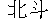
\includegraphics{Slovar/figs/beidou.pdf} angl. the Chinese asterism equivalent to the Big Dipper, labelling the Chinese satellite navigation system, also known as COMPASS or BeiDou-2}{kitajski sistem, poimenovan po ozvezdju Veliki voz, glede na ostale svetovne navigacijske satelitske sisteme temelji na podatkih lastnih geostacionarnih satelitov z oznako IGSO, v vzpostavljanju od 2015, trenutno (\today) v orbiti 21 zdravih od predvidenih 35 satelitov, stanje: {\footnotesize http://www.navipedia.org/index.php/Category:BEIDOU}}
	
	\entry{bias}{odstopanje, pristranskost}{angl.}{je sistematični pogrešek merilnega instrumenta (merilne verige), znan predznak; sistematični pogrešek pri merjenju globine z globinomerom povzročimo, če narobe izmerimo višinsko razliko med dnom oddajnika globinomera in dnom ladje oz. gredlja - ta razlika nam bo vedno za enako vrednost kvarila rezultate}
	
	\entry{Big Data}{način zbiranja podatkov}{angl. systems and software that analyse multiple data streams for insight}{sistemi in programi, ki z analizo raznovrstnih nizov podatkov iščejo nova spoznanja}
	
	\entry{bit}{enota za količino podatkov}{angl. a measure for the binary data quantity (\textit{see kilobit})}{količina binarnih podatkov}
	
	\entry{Bn}{radijska postaja}{angl. beacon}{ponavadi oddajna postaja}
	
	\entry{bps}{hitrost prenosa podatkov}{angl. bits per second}{en 1 bit na sekundo}
	
	\entry{brg}{kurz}{angl. bearing}{smer plovbe oz. kot med severom in izbrano smerjo}
	
	\entry{Broadcasting-satellite service}{javna satelitska storitev}{angl. a radiocommunication service in which signals transmitted or retransmitted by space stations are intended for direct reception by the general public}{javna radiokomunikacijska storitev v kateri so signali oddani ali prenešeni uporabnikom preko postaj v vesolju}
	
	\entry{Broadcasting service}{javna radijska storitev}{angl. a radiocommunication service in which transmissions are intended for direct reception by the general public}{javna radiokomunikacijska storitev v kateri so signali namenjeni vsem uporabnikom}
	
	\entry{byte}{količina podatkov}{angl. collection of bits that makes up a binary word}{skupek bitov, ki tvori binarno besedo, vsaj 8 bitov}
	
\end{multicols}

%----------------------------------------------------------------------------------------
%	SECTION C
%----------------------------------------------------------------------------------------

\section*{C}

\begin{multicols}{2}
	
	\entry{$^{\circ}$C}{zapis temperature}{angl. degrees Celsius}{zapis stopinj, ki imajo enoto $1/100$ intervala med temperaturo ledišča in vrelišča vode in ničlo pri ledišču vode}
	
	\entry{C/A code}{vrsta zaporedja}{angl. coarse acquisition code}{standardno psevdonaključno zaporedje GPS je zaporedje 1023 binarnih modulacij na nosilnem signalu GPS s frekvenco 1023 MHz, znano je pod imenom 'civilna koda', 'coarse'  pomeni grobo določitev položaja, 'acquisition' pa je izraz za določitev položaja iz vojaškega žargona. Vojaški sprejemniki GPS uporabljajo psevdonaključno zaporedje C/A za začetni grobi priklop na signal GPS, preden preidejo na višji nivo zaporedja P.}	
	
	\entry{carrier phase GPS}{vrsta rabe GPS}{angl.}{meritve GPS na podlagi faz nosilnih signalov ($L_1$ ali $L_2$ ali kombinacije obeh)}
	
	\entry{Cathode Ray Tube}{vrsta radarskega zaslona}{angl. CRT is a vacuum tube that contains one or more electron guns and a phosphorescent screen, and is used to display images. It modulates, accelerates, and deflects electron beam onto the screen to create the images. The images may represent electrical waveforms (oscilloscope), pictures (television, computer monitor), radar targets, or others.(wiki)}{katodna cev je vakuumirana elektronska cev, v kateri curki elektronov iz elektronskih topov zadevajo fosforescentni zaslon in puščajo na njem podobe. Podobe lahko ponazarjajo oblike električnih signalov (osciloskop), slike (televizija), radarski objekti in drugo.}
	
	
	\entry{celestial equator}{vrsta ekvatorja}{angl. The projection of Earth’s geographic equator onto the celestial sphere.}{projekcija ekvatorja Zemlje na neb$ \acute{e} $sno sfero. Manj kot 1 stopinjo stran od podaljšane osi od središča Zemlje proti severnemu geografskemu polu se na veliki oddaljenosti nahaja Severnica, zato jo jemljemo kar kot severni tečaj Zemljinega neb$ \acute{e} $snega koordinatnega sistema.}
	
	\entry{celestial sphere}{okvir neb$ \acute{e} $snega koordinatnega sistema}{angl. An imaginary rotating spherical shell around the Earth and concentric with it.}{navidezno vrteč se in oddaljen kroglast ovoj okoli Zemlje, z izhodiščem v središču Zemlje in severnim neb$ \acute{e} $snim polom trenutno v zvezdi Severnici (\textit{lat. stella polaris}). Zaradi precesije Zemlje s periodo $ 25.700 let $ namreč navidezno mirujoča polarna zvezda ni bila in ne bo vedno ista zvezda.}
	
	\entry{Centres Regionaux de Surveillance et de Sauvetage}{del sistema za nadzor in reševanje}{fr. CRSS}{regionalno središče za spremljanje in reševanje}
	
	\entry{Channel}{kanal}{angl. Ch}{frekvenčni pas elektromagnetnega spektra za izbran namen uporabe}
	
	\entry{Channel Navigation Information Service}{služba za pomoč pri navigaciji v Kanalu}{angl. CNIS helps vessels navigate safely and prevents collisions in the Dover Strait}{služba, ki neprestano oskrbuje z radijskimi in radarskimi informacijami, pomembnimi za navigacijo in preprečevanje trčenj v Rokavskem prelivu}		
	
	\entry{clock bias}{napaka merjenja časa}{angl.}{odstopanje med časom, ki ga kaže določena ura, in dejanskim univerzalnim časom (UT1)}
	
	\entry{Class A or B, AIS}{vrsta naprav AIS}{angl. Class of AIS installation}{vrsta naprav AIS: A za   velike ladje, B za plovila za kratkočasne dejavnosti}
	
	\entry{Coast Earth Station}{vrsta radijske postaje}{angl. CES, also Land Earth Station}{nepremična radijska postaja na kopnem, namenjena za storitve fiksnih satelitskih komunikacij ali včasih tudi nomadskih pomorskih satelitskih komunikacij, zagotavlja radijske zveze pomorskim nomadskim satelitskim storitvam.}
	
	\entry{Coast Guard}{obalna straža}{angl. CG}{služba za delo v priobalnem morju posamezne države}
	
	\entry{Coast Radio Station}{vrsta radijske postaje}{angl. a land station in the maritime mobile service, CRS}{kopenska postaja, ki omogoča pomorske nomadske komunikacije}
	
	
	\entry{Coded information}{način prenašanja informacij}{angl. information which is digitally coded within equipmnet by the user to provide information related to distress}{preden se informacija operaterja, npr. povezana s klicem v stiski, prenese naprej, se v radijski postaji digitalno kodira.}
	
	\entry{code phase GPS}{način rabe GPS}{angl.}{faza psevdonaključnega zaporedja C/A, meritve časov se izvajajo na podlagi merjenja faze zaporedja C/A}
	
	\entry{Comité International Radio-Maritime}{mednarodni odbor}{fr. CIRM}{odbor za radijske zveze v pomorstvu}
	
	\entry{Continious Wave telegraphy}{oznaka prekinjanega nosilnega signala}{angl. keying the transmitted signal, A1A}{oddajanje Morsejevih znakov samo z nosilnim signalom}
	
	\entry{continuity}{lastnost GNSS}{angl. The continuity of a system is the ability of the total system (comprising all elements necessary to maintain craft position within the defined area) to perform its function without interruption during the intended operation. More specifically, continuity is the probability that the specified system performance will be maintained for the duration of a phase of operation, presuming that the system was available at the beginning of that phase of operation.}{Neprekinjenost sistema kaže sposobnost celotnega sistema (vključuje vse elemente, ki položaj vozila ohranjajo v predvidenem območju), da opravlja svojo funkcijo brez prekinitev med nameravanimi operacijami. Podrobneje rečeno je razpoložljivost verjetnost, da bo izbrana lastnost sistema v eni fazi delovanja ostala v predpisanih mejah, če je bil sistem razpoložljiv na začetku te faze delovanja.}	
	
	
	%\entry{..}{}{angl.}{..}	
	
	\entry{Conventional Buoy Marking}{označevanje boj}{angl. CBM}{mednarodni dogovor označevanja pomorskih boj}
	%\entry{..}{}{angl.}{..}	
	
	\entry{COnvention on internationaL REGulations for preventing collisions at Sea}{mednarodni sporazum}{angl. COLREGS, 1972}{sporazum s pravili kako preprečevati trčenja na morju}
	
	
	\entry{Co-ordinate Conversion}{pretvarjanje zapisov med koordinatnimi sistemi}{angl. That process which changes co-ordinates produced using one system to conversion co-ordinates in another system.}{s pomočjo znanih odnosov med definiranimi koordinatnimi sistemi (izhodišče, osi, enote) transformiramo zapis v enem koordinatnem sistemu v drugega. Primer: transformacija iz krogelnega sistema $(\rho, \alpha, \varphi)$ v kartezični $(x,y,z)$ ali transformacija in projekcija iz svetovnega sestava WGS-84 $(\varphi, \lambda, h)$, na katerem je zasnovano podajanje položaja z GPS v državni koordnatni sestav D-96 v katerem geodetsko podajamo položaje $(Y,X,Z)$}	
	
	\entry{Co-ordinator surface search}{pooblaščena ladja za iskanje na morju}{angl. a vessel, other than rescue unit, designated to co-ordinate surface search and rescue operations within a specific search area}{ladja je pooblaščena za koordiniranje iskanja in reševanja, ni pa namenjena samemu reševanju}		
	
	
	\entry{Coronal Mass Ejection}{vrsta izbruha na Soncu}{angl. CME is	an outflow of plasma from or through the solar corona. CMEs are often, but not always, associated with erupting prominences, disappearing solar filaments, and/or flares.  CMEs vary widely in structure, density, and velocity.  Large and fast CMEs can approach densities of $ 10^{16} g$ and velocities of $ 2000 km/s $.  Earth impacting CMEs can result in significant geomagnetic storms.}{izredno velik izbruh plazme in nenadnega lokalnega preoblikovanja magnetnega polja iz Sončeve korone ali skozi njo.}
	
	\entry{correlation}{vrsta (matematičnega) postopka obdelave signalov}{angl. by shifting the replica GPS code the correlation can be get with the received GPS satellite code}{je matematični postopek, s katerim opišemo stopnjo ujemanja dveh enakih ali različnih signalov, ki sta med seboj fazno ali časovno zamaknjena. Stopnjo ujemanja v odvisnosti od faze opisuje korelacijska funkcija dveh periodičnih signalov.}
	%https://www.e-education.psu.edu/geog862/node/1756			
	
	\entry{COSPAS-SARSAT system}{satelitski sistem za posredovanje podatkov v stiski}{angl. a satellite-based search and rescue (SAR) distress alert detection and information distribution system, best known for detecting and locating emergency beacons activated by aircraft, ships and backcountry hikers in distress.}{v vozilu, plovilu ali pohodniku v nevarnosti se samodejno aktivira naprava, ki prek satelita obvesti center za posredovanje podatkov iskalcem ponesrečencev}
	
	\entry{coupling GNSS/INS}{način združevanja podatkov v enotno navigacijsko rešitev}{angl. GPS and inertial data coupling}{sklopitev GPS/INS ali INS/GPS pomeni, da navigacijski postopek kombinira podatke sprejemnika GPS in enote INS. Izraz GPS/INS ali INS/GPS pogosto zavaja, saj se zaradi 'tesnejše sklopitve rezultatov' v kombinacijo uvaja zgolj rezultate posameznih inercijskih merilnih enot in ne rezultatov, ki jih daje celotni (združeni) inercijski merilni sistem.}	
	
	%\item [sklopitev GPS/INS ali INS/GPS] pomeni, da navigacijski postopek kombinira podatke sprejemnika GPS in enote INS.  Izraz GPS/INS ali INS/GPS pogosto zavaja, saj se zaradi 'tesnejše sklopitve rezultatov' v kombinaciji nahaja zgolj IMU in ne celoten INS.
	
	% That process which changes co-ordinates produced using one system to conversion co-ordinates in another system, i.e. when using Loran-C changing from time differences (TDs) to geodetic co-ordinates. This could be achieved by interpolation on Loran-C overprinted charts or automatically by the Loran-C receiver.
	
	
	%\entry{Course Made Good}{vrsta kurza med odčitki GNSS}{angl. CMG}{kurz vzdolž loksodrome med dvema navigacijskima rešitvama položaja satelitskega navigacijskega sprejemnika}
	
	
	\entry{Course Over Ground}{kurz med odčitki GNSS}{angl. COG, direction of (the ship’s) movement relative to the Earth, measured on board (the ship).}{smer gibanja ladje glede na zemeljski koordinatni sistem, izmerjena na ladji}
	
\end{multicols}

%----------------------------------------------------------------------------------------
%	SECTION Č
%----------------------------------------------------------------------------------------

\section*{Č}

\begin{multicols}{2}
	
	\entry{Čajka}{vrsta hiperboličnega sistema}{angl. Chayka}{prvi LORAN-C sistem, ki so ga uvedli v nekdanji Sovjetski zvezi.}	
	
	\entry{čip}{binarni element, digit}{angl. chip, code chip}{košček zaporedja (kode) v navigacijskih sporočilih, ki sam ne prenaša informacije, ampak omogoča istovetnost (identifikacijo) satelitov; v elektronskih napravah pomeni čip tudi elektronski element - integrirano vezje, ki združuje v sebi množico miniaturnih polprevodniških elementov.}	
	
	
	%	\entry{..}{}{angl.}{..}
	
\end{multicols}	

%----------------------------------------------------------------------------------------
%	SECTION D
%----------------------------------------------------------------------------------------

\section*{D}


\begin{multicols}{2}
	
	\entry{dead reckoning, deduced reckoning}{način določanja položaja objekta}{angl.}{seštevna navigacija, pridobivanje informacij o premikanju s pomočjo meritev z inercijskimi senzorji. Prvi izraz je ponavadi napačno uporabljen, oba izraza v slovenščini nadomeščamo z besedno zvezo seštevna navigacija. Obstajata dve osnovni možnosti seštevne navigacije: 1. meritev pospeškov in kotnih hitrosti za posodabljanje podatka o položaju, 2. računanje položaja iz radijskih (CW) signalov zemeljskih oddajnikov. Zavedati se moramo, da točnost izračunov položaja s seštevno navigacijo zahteva periodično popravljanje rezultatov, perioda popravljanj pa je odvisna od kakovosti oz. od točnosti senzorjev.}
	
	\entry{Dead weight Tonnage}{oznaka obremenljivosti ladje}{angl. DWT}{tonaža ladje}
	
	\entry{decibel}{mera za delež moči, npr. sprejete moči glede na oddano moč}{angl. dB}{decibel je desetkratnik logaritma količnika dveh moči. V količniku pod ulomkovo črto je oddana moč, nad ulomkovo črto pa sprejeta moč.}	
	
	\entry{decibel watt}{normiran decibel, mera za delež moči}{angl. dBW}{decibel vat, desetkratnik logaritma količnika neke moči in moči $1W$.}
	
	\entry{decibel milliwatt}{normiran decibel, mera za delež moči}{angl. dBm}{decibel milivat, desetkratnik logaritma količnika neke moči in moči $1mW$.}
	
	%	
	
	\entry{declination}{pojem ali (1) iz neb$ \acute{e} $sne geografije ali (2) iz teorije uporabe magnetnega kompasa}{angl. (1) The angular distance of an astronomical body north (+) or south (-) of the celestial equator. (2) In geomagnetic applications, the angle between true north and the horizontal component of the local geomagnetic field.}{(1) kotna razdalja med objektom in neb$ \acute{e} $snim ekvatorjem, (2) kot med pravim meridianom in horizontalno komponento lokalnega geomagnetnega polja.}
	
	\entry{Degree of Freedom}{prostostne stopnje}{angl. Ship motions are defined by the six degrees of freedom that a ship, boat or any other craft can experience.}{Šest prostostnih stopenj je v treh dimenzijah za vsak masni objekt definiranih glede na smer objektovega gibanja; izhodišče koordinatnega sistema objekta sovpada z masnim središčem ali z osjo, okoli katere se objekt med gibanjem navidezno vrti; med prostostne stopnje spadajo premiki vzdolž vsake od treh glavnih osi (naprej-nazaj, levo-desno, navzgor-navzdol) in zavrtitve okoli teh treh osi.}
	
	
	
	%	\entry{..}{}{angl.}{..}
	%\item [zakasnitev, fazna] ({\em {phase delay}}) je v fazno linearnih sistemih (z neinvertirajočim ojačenjem) enaka grupni zakasnitvi oziroma tudi zakasnitvi sistema, za katerega je značilno, da njegov fazni zamik $\Phi$ linearno narašča s frekvenco $\omega$. Fazno zakasnitev v splošnem smislu izračunamo kot ulomek faznega zamika in frekvence z negativnim predznakom.
	
	%	
	
	\entry{delta Root-Mean-Square}{raztros okoli prave vrednosti}{angl.}{$\Delta$RMS, efektivna vrednost radialne razdalje velikega števila odčitkov do prave vrednosti (glej tudi istopomenko rms). Območje 2$\Delta$RMS po definiciji vsebuje 95 \%  vseh odčitkov. Elipsa  95 \% zaupanja predstavlja razširjeno območje standardne elipse zaupanja, povečane s faktorjem 2,447.}	
	
	%	\entry{..}{}{angl.}{..}	
	
	\entry{deviation, standard}{odstopanje}{angl. }{včasih poimenovan tudi odklon, izmerjena vrednost minus referenčna vrednost, primerjaj z ('error') merilni pogrešek; standardni odmik je zelo pogosta meja statistične razpršenosti, predstavlja kvadratni koren variance (glej tudi sopomenki RMS in dRMS).}
	
	\entry{deviation, standard of point's coordinates}{način podajanja natančnosti položaja}{angl.}{standardni odmik koordinat točke, standardni odmik (horizontalnih) koordinat točke, kvadratna sredina (kvadratni koren iz polovice vsote kvadratov standardnih odmikov obeh horizontalnih koordinat točke); je najenostavnejša skalarna mera točnosti horizontalnih koordinat točke.}
	
	\entry{deviation, standard of point's coordinates, generalized}{način podajanja natančnosti položaja}{angl.}{posplošeni standardni odmik koordinat točke, standardni odmik (horizontalnih) koordinat točke je geometrična sredina obeh polosi standardne elipse zaupanja (polmer kroga s površino, enako površini te elipse); gre za skalarno mero natančnosti horizontalnih koordinat točke, ki ji daje statistika prednost.}
	
	%\item [standardni odmik koordinat točke, posplošeni] standardni odmik (horizontalnih) koordinat točke je geometrična sredina obeh polosi standardne elipse zaupanja (polmer kroga s površino, enako površini te elipse); gre za skalarno mero natančnosti horizontalnih koordinat točke, ki ji daje statistika prednost  \cite{NavodiloGeodetom-2006}.
	
	%\item [standardni odmik koordinat točke] standardni odmik (horizontalnih) koordinat točke, kvadratna sredina (kvadratni koren iz polovice vsote kvadratov standardnih odmikov obeh horizontalnih koordinat točke); je najenostavnejša skalarna mera točnosti horizontalnih koordinat točke.
	
	%\item [standardni odmik] je zelo pogosta meja statistične razpršenosti, predstavlja kvadratni koren variance (glej tudi sopomenki RMS in dRMS)
	
	\entry{$D_G$}{razdalja med dvema tockama}{angl. distance between two points on a great circle, orthodromic distance}{razdalja vzdolž ortodrome, najkrajša pot med dvema točkama po površini krogle, ne upoštevaje poti, ki poteka skozi notranjost krogle}
	
	\entry{differential GPS}{diferencialni ameriški satelitski navigacijski sistem}{angl. DGPS}{način določanja položaja, hitrosti in časa s pomočjo satelitske navigacije in dodatne stalne postaje na Zemlji}
	
	\entry{differential GNSS}{diferencialni svetovni satelitski navigacijski sistem}{angl. DGNSS}{način določanja položaja, hitrosti in časa s pomočjo svetovne satelitske navigacije  in dodatne stalne postaje na Zemlji}		
	
	\entry{Digital Selective Call}{digitalizirani klic izbranega naslovnika}{angl. DSC}{tehnika prenašanja digitaliziranih sporočil, s katero po predpisih CCIR radijska oddajna postaja vzpostavi zvezo in prenese sporočilo drugi postaji ali skupini postaj}	
	
	\entry{Dillution of Precission}{podajanje teoretične negotovosti GNSS}{angl. DOP,  is a term used in satellite navigation and geomatics engineering to specify the additional multiplicative effect of navigation satellite geometry on positional measurement precision}{ DOP se nanaša na kakovost določitve položaja z GNSS; izraža razmerje med napako položaja sprejemnika GNSS in napako položajev satelitov – geometrijsko je to vrednost, ki je obratno sorazmerna volumnu štiristrane piramide, ki jo tvorijo sprejemnik in štirje sateliti, ki so v času meritev nad obzorjem najugodneje razporejeni.}	
	
	\entry{Distress Alerting}{hitro posredovanje alarma}{angl. rapid and successful reporting of a distress incident to a unit which can provide or co-ordinate assistance}{hitro in uspešen prenos poročila o dogodku s plovilom v stiski enoti, ki posreduje ali koordinira pomoč}	
	
	\entry{Distress Call}{klic v stiski}{angl. a part of the distress communication procedure, which includes a transmission of the distress-priority request message, and the reception of the Coast Earth Station answerback followed by the Rescue Co-ordination Centre Answerback.}{del komunikacijskega postopka v stiski, ki vključuje oddajo prioritetnega sporočila v stiski in sprejem odgovora obalne postaje (CES), ki mu sledi tudi odgovor središča za koordinacijo (RCC).}	
	
	\entry{Distress Channel}{vrsta kanala v stikski}{angl. an integrated channel between a ship in distress and Rescue Co-ordination Centre. The channel consists of of the ship's teletype or telephone set, Ship Earth Station, satellite channel, Coast Earth Station, land line and the end terminal at the Rescue Co-ordination Centre.}{združeni kanal za klic v stiski, ki ga sestavljajo telegrafska ali telefonska naprava, ladijska zemeljska postaja, satelitska zveza, kopenska zemeljska postaja, naprava v centru za koordinacijo reševanj za sprejem omenjenih zvez in obenem tudi s kopensko povezavo.}	
	
	\entry{Distress Message}{vrsta sporočila}{angl. the contents is defined by the Radio Regulations, RR3093, and may be formatted as defined by INMARSAT and IMO GMDSS for the Distress Message Generator (INMARSAT Ship Earth Station Technical Bulletin No 19, February, 1987 and Annex IV to COM 29/10)}{ vsebino sporočila določajo posebna pravila RR3093, sporočilo je lahko oblikovano po definicijah INMARSAT in IMO GMDSS za generator sporočil (Distress Message Generator)}	
	
	\entry{Distress Priority Request Message}{vrsta sporočila}{angl. a ship to shore request message containing priority indication 3, the highest priority of ship to shore calls.}{ zahteva z najvišjo prioriteto, ki jo v telefoniji pošlje ladijska postaja zemeljski postaji}	
	
	\entry{Doppler shift}{pojav zaradi premikanja}{angl. A change in the perceived frequency of a radiated signal caused by motion of the source relative to the observer.}{Dopplerjev pojav pomani spremembo zaznavane frekvence zaradi relativnega premikanja izvora glede na opazovalca oz. poslušalca.}
	
	
	\entry{Dual Side Band}{način v telefoniji}{angl. DSB}{delo z obema bočnima pasovoma}	
	
\end{multicols}

%----------------------------------------------------------------------------------------
%	SECTION E
%----------------------------------------------------------------------------------------

\section*{E}

\begin{multicols}{2}
	
	%ecliptic	The great circle made by the intersection of the plane of the Earth’s orbit with the celestial sphere. (Less properly, the apparent path of the Sun around the sky during the year.)			
	
	\entry{ecliptic}{ovalna črta}{angl. The great circle made by the intersection of the plane of the Earth’s orbit with the celestial sphere. (Less properly, the apparent path of the Sun around the sky during the year.}{sklenjena črta, ki nastane, ko ravnina Zemljine tirnice preseka nebesno sfero, manj točno ekliptika pomeni navidezno pot Zemlje okoli Sonca.}			
	
	\entry{e.g.}{npr.}{angl. example giving}{na primer}
	
	\entry{EIRP}{moč na anteni}{angl. 1) Effective Isotropic Radiated Power, 2) Eqiuvalent Isotropically Radiated Power}{1) 2) zmnožek dovedene moči anteni in dobitka antene, v izbrani smeri, glede na moč, bi jo izsevala (izotropna) antena (v dBW). Izotropna antena seva v vse smeri enako moč.}
	
	
	\entry{Electronic Chart Display and Information System}{vrsta geografskega informacijskega sistema (GIS)}{angl. ECDIS,  displays the information from electronic navigational charts (ENC) or Digital Nautical Charts (DNC) and integrates position information from position, heading and speed through water reference systems and optionally other navigational sensors. Other sensors which could interface with an ECDIS are radar, Navtex, Automatic Identification Systems (AIS), and depth sounders.}{ informacijski sistem ECDIS sestavlja elektronska karta, ki vključuje navigacijsko rešitev (položaj, smer, hitrost skozi vodo), lahko tudi druge dopolnilne informacije; dopolnilne informacije dajejo: radar, Navtex, AIS, in globinomeri.}
	
	%	\entry{..}{}{angl.}{..}
	%	\entry{..}{}{angl.}{..}
	
	\entry{Electromagnetic Spectrum}{skupno ime za vse frekvence znanih elektromagnetnih sevanj}{angl. The electromagnetic spectrum extends from below the low frequencies used for modern radio communication to gamma radiation at the short-wavelength (high-frequency) end, thereby covering wavelengths from thousands of kilometers down to a fraction of the size of an atom. Visible light lies toward the shorter end, with wavelengths from 400 to 700 nanometres. The limit for long wavelengths is the size of the universe itself, while it is thought that the short wavelength limit is in the vicinity of the Planck length, (wiki).}{v valovne dolžine preračunane frekvence spektra segajo od najdaljših, ki so lahko dolge kot premer vesolja $8,8\cdot10^{26}m$ do najkrajših znanstveno potrjenih $10^{-16}m$ in teoretično še možnih, ki jih ponazarja Planckova dolžina $1,6\cdot10^{-35}m$; gama žarki imajo valovno dolžino reda $10^{-12}m$ oz. 1pm, vidna svetloba reda $10^{-6}m$ oz. $1\mu m$, radijski in mikrovalovi od $1mm$ do $100m$. http://htwins.net/scale2/}%({\href{https://en.wikipedia.org/wiki/Electromagnetic_spectrum}{\textit{wiki}})}}
	
	\entry{ellipse of trust, standard}{način zapisa nedoločenosti rezultata položaja}{angl. }{standardna elipsa zaupanja je običajen način podajanja razpršenosti dvorazsežne populacije (npr. natančnosti para horizontalnih koordinat). Standardna elipsa zaupanja je podana s tremi parametri: veliko polosjo elipse ($a$), malo polosjo elipse ($b$) ter azimutom velike polosi ($\Theta$); gre za elipso, znotraj katere se nahaja 39,4 \% vseh parov slučajnih spremenljivk iz dvorazsežne populacije (npr. parov koordinat točke)}
	
	\entry{ellipsoid}{geometrijsko telo}{angl.}{geometrijsko telo, katerega ravninski preseki vzdolž ene osi so elipse, ravninski preseki vzdolž ostalih osi so elipse ali krogi (rotacijski elipsoid).}
	
	\entry{Emergency Position-Indicating RadioBeacon}{naprava, katere vklop izzove reševanje}{angl. EPIRB}{postaja v mobilni enoti (plovilu), ki se v nevarnosti samodejno ali ročno vključi, s po celem svetu razširjenim sistemom COSPAS-SARSAT pošilja podatek o položaju ponesrečencev, položaj je sistem nekdaj določal s pomočjo Dopplerjevega pojava (oddajanje na stalni frekvenci, sateliti pa stalno potujejo), dandanes pa s pomočjo vgrajenega sprejemnika GPS; naprava sporoča položaj plovila v nevarnosti iskalnim ter reševalnim ekipam.}
	
	\entry{e-navigation}{sodoben način navigacije}{angl. }{navigacija s pomočjo načina BigData, za katerega je potrebna povezava z medomrežjem, podrobneje na: {\scriptsize http://www.e-navigation.com/p/deep-sea-connectivity---no-longer-sci-fi}}	
	
	\entry{enhanced-Loran}{način radijske terestrične navigacije}{angl. e-Loran, the latest in the series of low frequency, LOng-RAnge Navigation systems. eLoran evolved from Loran-C in response to the 2001 Volpe Report on GPS vulnerability.}{Dodatni kanali predvsem za prenos stanja atmosfere v območju razširjanja elektromagnetnih valov omogočajo e-Loran-u večjo natančnost in dodatne možnosti uporabe glede na Loran-C, kar omogoča e-Loran-u, da ga lahko uporabljamo kot nadomestni sistem ob izpadu satelitske navigacije.}	
	
	\entry{ephemerides}{tabele z vrisanimi položaji satelitov oz. nebesnih teles v izbranem času}{angl. ephemeris}{na efemeridah lahko določimo položaj narisanih nebesnih teles glede na naše opazovališče v podanem časovnem obdobju. preglednica z zabeleženimi napovedanimi položaji nebesnih teles {\bf v koordinatnem sistemu ITRS ali ICRS} za določeno časovnno obdobje (vsaj za 1 h), vrednosti so zapisane v dvojiškem sistemu z 32 biti, ki so kot 'broadcast ephemerides' del podatkov v sporočilu s satelita GPS sprejemniku (negotovost položaja satelita reda velikosti 1 m) ali pa jih za zelo natančne naknadne obdelave kot 'precise ephemerides' (negotovost med 0,05 m in 0,20 m) uporabnik lahko dobi od IGS.}
	
	
	\entry{epoch}{referenčno časovno obdobje}{angl.}{časovno obdobje, v katerem sprejemnik GNSS opravi en izračun položaja in koordinate in za katerega tudi izpiše vrednost opazovanja oz. izmere na izhodni enoti. Epoha lahko znaša od delčka sekunde (za kinematična opazovanja, gibanja hitrih objektov, na primer vozil) do meseca, leta (za kinematična opazovanja gibanja počasnih objektov, na primer litografskih plošč).}
	
	\entry{error, measurement}{odstopanje odčitka}{angl.}{merilni pogrešek, izmerjena vrednost minus prava vrednost, v praksi namesto prave uporabljamo dogovorjeno pravo vrednost}
	
	\entry{Estimated Time of Arrival}{podatek, pomemben za načrtovanje plovbe}{angl. ETA}{ocenjen čas prihoda ladje v pristanišče}
	
	\entry{Estimated Time of Departure}{podatek, pomemben za načrtovanje plovbe}{angl.ETD}{ocenjen čas odhoda ladje iz pristanišča}
	
	\entry{European Geostationary Navigation Overlay Service}{evropski, na GPS in GLONASS vezan sistem satelitske navigacije}{angl. EGNOS is the European Satellite Based Augmentation System (SBAS) and was certified for civil aviation in March 2011.}{sistem geostacionarnih satelitov za določanje popravkov GPS in GLONASS. Preizkusni EGNOS \textit{System Test Bed} deluje od leta 2001; v vesolju \textit{Integration Test SIS} od aprila 2003; preizkusno obdobje operabilnosti (\textit{Oper. Eval. Phase}) od 2004; uradno v brezplačni javni uporabi (\textit{Open Service}) od 1. oktobra 2009 za vse oblike uporabe, ki ne vplivajo na varnost ljudi; od marca 2011 je potrjen tudi za uporabo v letalstvu.}		
	
	
	\entry{European Terrestrial Reference System 89}{referenčni geodetski datum}{angl. ETRS 89}{kratica imena evropskega terestričnega referenčnega sistema iz leta 1989; gre za evropski geocentrični geodetski datum oz. elipsoid, sprejet s strani EUREF; temelji na GRS 80; letnica predstavlja trenutek oziroma epoho (1989,0), v kateri je ta geodetski datum sovpadal z ITRS 89; je temelj (novega) slovenskega koordinatnega sistema z oznako ESRS/D96.}
	
	
	%\item [standardna elipsa zaupanja] je običajen način podajanja razpršenosti dvorazsežne populacije (npr. natančnosti para horizontalnih koordinat). Standardna elipsa zaupanja je podana s tremi parametri: veliko polosjo elipse ($a$), malo polosjo elipse ($b$) ter azimutom velike polosi ($\Theta$); gre za elipso, znotraj katere se nahaja 39,4 \% vseh parov slučajnih spremenljivk iz dvorazsežne populacije (npr. parov koordinat točke); glej \cite{NavodiloGeodetom-2006} in poglavje \ref{SubSec_2D3DMereTocnosti}.	
	
\end{multicols}

%----------------------------------------------------------------------------------------
%	SECTION F
%----------------------------------------------------------------------------------------

\section*{F}

\begin{multicols}{2}
	
	\entry{$^\circ$F}{zapis temperature}{angl. degrees Fahrenheit}{stopinje po Fahrenheitovi lestvici}	
	
	\entry{F1B}{način prenosa podatkov}{angl. telegraphy using frequency modulation: Narrow Band Direct-Printing (Telex)}{telegrafija, ki uprablja frekvenčno modulacijo (NBDP oz. teleks)}	
	
	\entry{F1D}{način prenosa podatkov}{angl. data transmission using frequency modulation, with a single channel containing digitized data without the use of a modulating sub-carrier}{prenos podatkov, ki iporablja frekvenčno modulacijo na enem kanalu, digitalizirani podatki, vendar brez uporabe pasu pod frekvenco nosilnega signala}
	
	\entry{F2B}{način prenosa sporočil}{angl. telegraphy using frequency modulation with a single channel containing digitized data with the use of a modulating sub-carrier, for automatic reception}{prenos podatkov, ki iporablja frekvenčno modulacijo na enem kanalu, digitalizirani podatki, vendar z uporabo pasu pod frekvenco nosilnega signala, namenjenega za samodejni sprejem}
	
	%	\entry{F2C}{način prenosa sporočil}{angl. }{}	
	%	\entry{F2D}{način prenosa sporočil}{angl. }{}
	%	\entry{F2C}{način prenosa sporočil}{angl. }{}
	%	\entry{F3C}{način prenosa sporočil}{angl. }{}
	%	\entry{F3E}{način prenosa sporočil}{angl. }{}
	
	\entry{failure}{napaka}{angl.The unintended termination of the ability of a system, or part of a system, to perform its required function.}{stanje nehotenega prenehanja zmožnosti sistema, da opravlja predvidene funkcije, če je vključen človek, napako imenujemo \textit{pomota}.}
	
	\entry{failure rate}{pogostnost napake}{angl.The average number of failures of a system, or part of a system, per unit time.}{povprečno število napak sistema ali njegovega dela na časovno enoto.}
	
	\entry{Feeder Link}{vrsta servisne zveze zemlja - satelit}{angl. a radio link from an earth station at a specified fixed point to a space station or vice  versa, conveying information for a space radiocommunication service other than for the fixed satellite service}{radijska zveza, ki povezuje fiksno zemeljsko postajo in postajo v vesolju ali obratno, posredovanje informacij za vse vrste vesoljskih radiokomunikacijskih storitev, razen za storitve fiksne satelitske storitve.}
	
	\entry{File Transfer Protocol}{način prenosa sporočil}{angl. FTP (Internet)}{standardni način medomrežnega prenosa podatkov}		
	
	\entry{fix, position}{odčitek položaja v nekem trenutku}{angl. }{praviloma en podatek o položaju z zemljepisno širino, dolžino, višino (nad referenčnim elipsoidom), geodetskim datumom, vključujoč tudi podatek o času zajema teh informacij.}	
	
	\entry{Fixed Satellite Service}{vrsta satelitskih podatkovnih zvez}{angl. FSS}{a radio-communication service between earth stations at given positions, when one or more satellites are used; the given position may be a specified fixed point or any fixed point within specified areas; in some cases this service includes satellite-to-satellite links, which may also be operated in the inter-satellite service; the fixed-satellite service may also include feeder links for other space radiocommunication services.}{storitev radijskih zvez med zemeljskimi postajami, v katerega je vključen tudi vsaj en satelit; vključuje tudi med-satelitske zveze.}
	
	\entry{Forward Error Correction}{zagotavljanje pravilnega prenosa sporočil}{angl. FEC}{metoda za nadzorovanje napak v sporočilih na zašumljenih in nezanesljivih zvezah. Temelji na dodanih znakih v sporočilu oz. redundanci, zaradi katerih lahko po tej metodi prenosna naprava sama prepozna del napak, brez potrebe po ponavljanju sporočil.}
	
	
	\entry{F region}{plast ionosfere}{angl. F region, the upper region of the ionosphere, above approximately 160 km altitude.  F region electron densities are highly variable, depending on the local time, solar activity, season, and geomagnetic activity. The F region contains the Fl and F2 layers. The F2 layer is more dense and peaks at altitudes between 200 and 600 km. The Fl layer, which forms at lower altitudes in the daytime, has a smaller peak in electron density.}{gornja plast ionosfere, združuje plasti F1 in F2; F2 je gostejša na višinah med $ 200 $ in $ 600 km $.}
	
	\entry{Frequency Modulation}{način prenosa sporočil}{angl. FM}{frekvenčna modulacija}
	
	\entry{Frequency-Shift Keying}{način prenosa sporočil}{angl. FSK}{frekvenčno kodiranje}
	
	%	\entry{..}{}{angl.}{..} 
	
\end{multicols}

%----------------------------------------------------------------------------------------
%	SECTION G
%----------------------------------------------------------------------------------------

\section*{G}

\begin{multicols}{2}
	
	\entry{GaAs}{polprevodna spojina}{angl.}{snov, uporabna za izdelavo monolitnih mikrovalovnih elementov (Gunnovih diod), svetlečih infrardečih diod, laserskih diod in sončnih celic}	 
	
	\entry{GAGAN}{od GPS odvisni navigacijski sistem}{angl. GPS and GEO Augmented Navigation (Indian WAAS)}{indijski radijski navigacijski sistem z lastnimi sateliti v geostacionarni orbiti}
	
	\entry{Galileo}{eden od svetovnih neodvisnih satelitskih radijskih navigacijskih sistemov}{angl. European GNSS (GNSS-2)}{evropski sistem, del GNSS, upravlja ga evropska Agencija za GNSS (GSA), stanje: {\footnotesize http://www.navipedia.org/index.php/Galileo in https://www.gsc-europa.eu/system-status/Constellation-Information}}
	
	\entry{GDOP}{vrsta nenatančnosti določanja položaja GNSS}{angl. geometric dilution of precision}{faktor, za katerega sta poslabšani točnost določanja položaja 3D in časa zaradi geometrijskih razlogov.}
	
	\entry{geodetic accuracy}{vrsta točnosti položaja}{angl. The accuracy of a position with respect to the geodetic coordinates of the earth}{točnost podajanja položaja glede na zemeljske geodetske koordinate (definicija IMO)}
	
	\entry{geodetic datum}{nabor parametrov}{angl. A set of parameters specifying the reference coordinate system used for geodetic control in the calculation of coordinates of points on the earth}{(nabor parametrov (referenčnega elipsoida), ki natančno definirajo referenčni koordinatni sistem za geodetski nadzor nad preračunavanjem koordinat točk na Zemlji. Geodetski datum predstavlja zvezo med referenčnim terestričnim in referenčnim lokalnim koordinatnim sistemom, v katerem so narisane lokalne karte oz. zemljevidi. Datum sestavlja nabor dogovorjenih transformacij. (definicija ISO)}
	
	\entry{geodetic latitude}{geodetska širina}{angl. Angular distance between the plane of the geodetic equator and the normal to a point on the earth ellipsoid.}{kot med ekvatorialno ravnino in pravokotnico na zemeljski elipsoid iz dane točke.}
	
	\entry{geodetic longitude}{geodetska dolžina}{angl. Angular distance between the plane of the geodetic prime meridian and the plane of a point’s geodetic meridian.}{kot med ravnino prvega geodetskega meridiana in ravnino geodetskega meridiana skozi dano točko.}
	
	\entry{geographic accuracy}{vrsta točnosti določanja položaja}{angl. The accuracy of a position with respect to the geographic coordinates of the earth.}{točnost podajanja položaja glede na zemeljske geografske koordinate (definicija IMO).}
	
	\entry{geographic information system}{vrsta informacijskega sistema}{angl. a system designed to capture, store, manipulate, analyze, manage, and present all types of spatial or geographical data, GIS}{je informacijski sistem, ki združuje, shranjuje, popravlja, analizira, izmenjuje med zainteresiranimi in prikazuje geografske informacije. Rešitve GIS so orodja, ki omogočajo uporabnikom, da opravljajo interaktivne poizvedbe, analizirajo podatke o prostoru, popravljajo podatke in karte ter predstavljajo rezulate vseh teh dejavnosti.}
	
	\entry{geoid}{po težnostnem polju Zemlje oblikovano telo}{angl.}{predstavlja ekvipotencialno ploskev težnostnega polja Zemlje, ki v največji možni meri predstavlja približek srednje višine gladine morja. Površina geoida je povsod pravokotna na smer težnostnega pospeška, zaradi česar je telo geoida nepravilne oblike. Zbirka meritev težnostnega polja Zemlje vsebuje anomalije težnostnih polj oceanov iz satelitskih meritev višine (satelitska altimetrija), modeliranje potenciala težnostnega polja in rezultate površinskih opazovanj težnosti na kopnem.}
	
	\entry{geomagnetic elements}{kvantitativni opis Zemeljskega magnetnega polja v izbrani površinski točki}{angl. The components of the geomagnetic field at the surface of the Earth. These elements are usually denoted as in the literature: \textbf{X}-the geographic northward component, \textbf{Y} -the geographic eastward component, \textbf{Z}-the vertical component, reckoned positive downward, \textbf{H}-the horizontal intensity, of magnitude $ \sqrt{x^2 + y^2} $, \textbf{F}-the total intensity $ \sqrt{H^2 + Z^2} $, \textbf{I}-the inclination (or dip) angle, $ arctan(Z/H) $, \textbf{D}-the declination angle, measured from the geographic north direction to the H component direction, positive in an eastward direction; $ D = arctan (Y/X) $. The geomagnetic northward and geomagnetic eastward components are sometimes called the H and D components. The H axis direction is defined by the mean direction of the horizontal component relative to the geomagnetic north by using the small-angle approximation. Thus the $D =  H \cdot \Delta D $ (the declination angle relative to geomagnetic north, expressed in radians).}{v literaturi ponavadi navajajo elemente vektorja gostote magnetnega pretoka zemeljskega magnetnega polja: komponenta \textbf{X} kaže v smer geografskega severa, \textbf{Y} v smer geografskega vzhoda, \textbf{Z} proti središču Zemlje, horizontalna komponenta \textbf{H} je geometrijska vsota X in Y, kot inklinacije oz. nagiba \textbf{I} ter kot deklinacije \textbf{D} oz. smerjo komponente H, ki jo v pomorstvu imenujemo \textit{\textbf{variacija}}, izračunamo po gornjih formulah;  D je pozitivna, če je Y pozitiven. Na bitvi avstrijskega pomola ($ 45,5157^{\circ} N, 13,5778^{\circ} E $)  smo 10. oktobra 2016 z modelom WMM2015 določili  $ D = 3,31^{\circ} E  \pm 0,34^{\circ} $  pri lezenju $ 0,11^{\circ} E$ na leto.} 
	
	%PODATKI:  www.ngdc.noaa.gov/geomag/declination.shtml 
	% Koliko znaša deklinacija v izbrani točki lahko izračunamo: 
	%http://www.ngdc.noaa.gov/geomag-web/#declination
	
	%
	
	
	\entry{geomagnetic field}{magnetno polje Zemlje}{angl. The magnetic field in and around the Earth. The intensity of the magnetic field at the Earth’s surface is approximately 32,000 nT at the equator and 62,000 nT at the north pole (the place where a compass needle points vertically downward). The geomagnetic field is dynamic and undergoes continual slow secular changes as well as short-term disturbances (see geomagnetic activity). The geomagnetic field can be approximated by a centered dipole field, with the axis of the dipole inclined to the Earth’s rotational axis by about 11.5 degrees. Geomagnetic dipole north is near geographic coordinate 79 degrees N and 71 degrees W (near Thule, Greenland), and dipole south is near 79 degrees S and 110 degrees E (near Vostok, Antarctica). The observed or dip poles, where the magnetic field is vertical to the Earth’s surface, are near 77 degrees N and 102 degrees W, and 65 degrees S and 139 degrees E. The adopted origin of geomagnetic longitude is the meridian passing through the geomagnetic poles (dipole model) and the geographic south pole. (See also corrected geomagnetic coordinates.)}{magnetno polje okoli Zemlje; gostota magnetnega pretoka na površini znaša na ekvatorju približno $ 32\mu T$, na severnem polu $ 62\mu T$ (kraj, kjer se kompasova igla odklanja navpično). Os geomagnetnega dipola je za približno 11,5 stopinj nagnjena od rotacijske osi Zemlje, severni krak dipola je na 79 N in 71 W (Thule, Grenlandija), južni pa 79 S, 110 E (Vostok, Antarktika). Območji, v katerih gostota magnetnega pretoka kaže navpično na površino Zemlje, sta 77 stopinj N, 102 stopinj W in 65 stopinj S in 139 stopinj E.} 
	
	\entry{geosynchronous altitude}{višina, na kateri je kotna hitrost gibanja nad ekvatorskih objektov enaka kotni hitrosti Zemlje}{angl. Term applied to any equatorial satellite with an orbital velocity equal to the rotational velocity of the Earth. The geosynchronous altitude is near 6.6 Earth radii (approximately $ 36,000 km $ above the Earth’s surface). To be geostationary as well, the satellite must satisfy the additional restriction that its orbital inclination be exactly zero degrees. The net effect is that a geostationary satellite is virtually motionless with respect to an observer on the ground.}{geosinhronska višina je približno 6,6 polmerov Zemlje (približno $ 36.000 km $); če želimo, da satelit popolnoma obmiruje, da je njegova hitrost glede na opazovalca na površini Zemlje enaka 0, mora biti nagnjenost površine satelitove tirnice glede na ekvatorialno ravnino Zemlje (inklinacija tirnice) enaka 0 stopinj.} 
	
	\entry{GEostationary Orbit}{eno od območij višin tirnic satelitov}{angl. GEO, among satellite operators known geosynchronous heights $ 35.786km $ (orbiting time the same as Earth rotation).}{območje satelitskih tirnic na geosinhronskih višinah $ 35.786km $ (obhodni čas enak enemu obratu Zemlje okoli svoje osi).}
	
	\entry{gimbaled inertial system}{vrsta pritrditve inercijskega senzorja}{angl. gyroscopically stabilized inertial system}{giroskopsko stabilizirani sistem, s kardanskim sklopom med objektom in inercijskim instrumentom omogočajo instrumentom, da ostanejo usmerjeni vedno v prvotno nastavljeno smer, kljub obračanju ploščadi oz. objekta.} 
	
	%\item [sistemi, giroskopsko stabilizirani]  (ang.  'gimbaled') s kardanskim sklopom med platformo in geofizikalnim merilnim instrumentom omogočajo pospeškometrom, da ostanejo usmerjeni vedno v prvotno nastavljeno smer, kljub obračanju platforme (geofizikalnega merilnega instrumenta).	 
	
	\entry{Global Positioning System}{prvi od polno delujočih svetovnih neodvisnih satelitskih radijskih navigacijskih sistemov}{angl. GPS, a space-based radionavigation system owned by the United States government and operated by the United States Air Force, All satellites broadcast at the same frequencies, encoding signals using unique code division multiple access (CDMA). Although usually not formed explicitly in the receiver processing, the conceptual time differences of arrival (TDOAs) define the measurement geometry. Each TDOA corresponds to a hyperboloid of revolution. }{ameriški sistem, del GNSS, upravljajo ga letalske sile ZDA, stanje: {\footnotesize http://www.gps.gov/}}
	
	\entry{GLONASS}{eden od polno delujočih svetovnih neodvisnih satelitskih radijskih navigacijskih sistemov}{rus. 
\includegraphics{Slovar/figs/glonass.pdf} angl. a global satellite navigation system, providing real time position and velocity determination for military and civilian users, using frequency division multiple access (FDMA)}{ruski sistem, del GNSS, upravljajo ga ruske vesoljske sile, stanje: {\footnotesize https://www.glonass-iac.ru/en/}}
	
	\entry{gnomon}{del sončne ure, senčnica}{angl. the projecting piece on a sundial that shows the time by the position of its shadow.}{palica oz. kazalec, ki ob Sončevem obsevanju meče senco na vodoravno ploščo}	
	
	\entry{governor}{regulator dovoda goriva v glavni motor}{angl.}{regulator hitrosti vrtenja glavnega ladijskega motorja, nekdaj s centrifugalnim, zdaj večinoma s hidrostatičnim elementom za vzrževanje željene hitrosti}	
	
	\entry{GPS initialization}{ena od dejavnosti natančnih sprejemnikov GPS}{angl.}{inicializacija GPS, visoka kakovost določitve koordinat na osnovi faznih opazovanj temelji na zanesljivi določitvi števila celih valov. Pri kinematičnih metodah je neznano število celih valov določeno po inicializaciji v začetnem trenutku opazovanj in je konstantno v času neprekinjenih opazovanj. V primeru prekinitve sprejemanja signalov (npr. ovire) je treba inicializacijo ponoviti (tj. ponovno določiti neznano število celih valov).}
	
	
	
\end{multicols}	

%----------------------------------------------------------------------------------------
%	SECTION H
%----------------------------------------------------------------------------------------

\section*{H}

\begin{multicols}{2}
	
	
	\entry{heading}{os objekta 'naprej'}{angl.}{os v smeri gibanja objekta, $u_x$, pravokotna na osi 'athwart' in 'heave'}	 
	
	\entry{heave}{os objekta 'navzgor'}{angl.}{vzdolž (navpične) osi $u_z$, pravokotna na osi 'naprej' ('heading') in 'vstran' 'athwart'}	 
	
	\entry{heel}{mirovna lega nagnjene osi ladje}{angl. Heel refers to an offset that is intentional or expected, as caused by wind pressure on sails, turning, or other crew actions. (wiki)}{nagnjenost, če je mirujoča ladja zaradi zunanjih ali notranjih vplivov nagnjena okoli osi premec-krma.}	
	
	\entry{High Troughput Satellite}{vrsta satelitskih podatkovnih zvez}{angl. HTS, classification for communications satellites that provide at least 2, though usually by a factor of 20 or more, the total throughput of a classic FSS satellite for the same amount of allocated orbital spectrum thus significantly reducing cost-per-bit.}{vrsta podatkovnih zvez, ki zagotavljajo vsaj dvakrat in celo več kot dvajsetkrat višje hitrosti prenosa kot klasične zveze FSS na enaki pasovni širini znotraj pasu Ku, kar bistveno zmanjša stroške na prenešen bit podatkov. V pomorski praksi HTS omogočajo sateliti Inmarsat Global Xpress.}
	
\end{multicols}	

%----------------------------------------------------------------------------------------
%	SECTION I
%----------------------------------------------------------------------------------------

\section*{I}

\begin{multicols}{2}	
	
	\entry{inclination of the geomagnetic field}{nagib vektorja $\vec{B} $}{angl. The angle between the local geomagnetic field density $\vec{B} $ direction and the horizon. (See geomagnetic elements.)}{nagnjenost lokalnega vektorja $\vec{B} $ pod ali nad vodoravno (tangencialno) ravnino v dani točki.} 
	%	\entry{..}{}{angl.}{..} 
	
	
	\entry{inertial navigation}{vrsta navigacijskih tehnik}{angl.}{inercijska navigacija temelji na zaznavanju linearnih pospeškov in kotnih zasukov relativno na inercijski sistem, na njej temelji seštevna navigacija z akumuliranjem podatkov s senzorjev v računalniku.}
	
	\entry{inertial frame}{vrsta koordinatnega sestava}{angl.}{sistem koordinat, v katerem je pospešek zanemarljiv - objekt miruje ali se giblje s konstantno hitrostjo. Primer inercijskega sestava je sestav vrteče se Zemlje.}
	
	\entry{Inertial Measurement Unit}{vrsta merilne naprave}{angl. IMU}{Inercijska merilna enota je skupina instrumentov (pospeškometrov in žiroskopov) za merjenje linearnega pospeška vzdolž treh osi in kotne hitrosti okoli treh osi.  IMU vsebuje senzorske elemente, elektroniko, in ponavadi procesor (računalnik), ki vodi kalibracijo ter kompenzacijo odstopanj senzorjev.}
	
	\entry{Inertial Navigation System}{vrsta navigacijskega sistema}{angl. INS}{inercijski navigacijski sistem je sistem, ki deluje po načelih seštevne navigacije, samovodljivi sistem, popolnoma neodvisen od zunanjih vizualnih in elektronskih informacij, sestavlja ga poseben žiroskopsko stabilizirani (ang.  'gimballed') ali magnetometrsko/giroskopsko stabilizirani (ang.  'strapdown') merilnik z nepomičnimi senzorji, ki merijo pospeške in kotne hitrosti v oseh izbranega koordinatnega sistema. INS poleg IMU vsebuje tudi računalnik za izvajanje seštevne navigacije iz rezultatov IMU (določanje težnostnega pospeška in dvojno integriranje za zagotavljanje ocene položaja merilnega instrumenta). V splošni rabi izraz INS povzema vse pojme, povezane z inercijsko navigacijo.}
	
	\entry{Integrated Navigation System}{več-orodni navigacijski sistem}{angl. INS, a system in which the information from 2 or more navigation aids is combined in a symbiotic manner to provide an output which is superior to any one of the component aids (IMO).}{združeni navigacijski sistem je sistem, v katerem se ves čas meritve (opazovanja) kombinirajo informacije z dveh ali večih navigacijskih orodij za zagotovitev izhodnih vrednosti, ki so po točnosti in zanesljivosti nadrejene vrednostim kateregakoli od posameznih uporabljenih orodij (definicija IMO). }
	
	\entry{integrity}{zmožnost sistema}{angl. Integrity is the measure of the trust that can be placed in the correctness of the information supplied by a navigation system. Integrity includes the ability of the system to provide timely warnings to users when the system should not be used for navigation.}{Integriteta je zmožnost sistema, da s samopreverjanjem zagotavlja uporabnikom opozorila o obdobjih, ko ne sme biti uporabljan za navigacijo (definicija IMO). Integriteta je mera, koliko zaupamo informaciji, ki nam jo daje navigacijski sistem. Integriteta vključuje sposobnost sistema, da v primernem času uporabniku zagotavlja opozorila, kdaj sistema ne sme uporabljati za navigacijo.}
	
	\entry{integrity risk}{verjetnost nezaznanega prestopa nastavljenega praga}{angl. Probability that a user will experience a position error larger than the threshold value without an alarm being raised within specified time to alarm at any instant of time at any location within the coverage area (IMO)}{verjetnost dogodka, ko bo uporabnik sistema nevede določil položaj z napako, večjo kot znaša dopustna (pričakovana) vrednost napake, ker ga sistem v dogovorjenem času od nastanka vzroka za napako na napako ni opozoril. Sistem zagotavlja informacije v predpisanem geografskem območju nadzora (definicija IMO). Značilna vrednost omenjenega tveganja je $10^{-7}$.}
	
	\entry{International Maritime Organization}{mednarodna organizacija}{angl. IMO}{mednarodna pomorska organizacija s sedežem v Londonu.}
	
	\entry{the Internet of Things at Sea}{način dostopa ladij do medomrežja}{angl. IoTs, global maritime network infrastructure interlinking physical and virtual objects through the Internet.}{infrastruktura svetovnega pomorskega omrežja, ki povezuje fizične in navidezne objekte s pomočjo medomrežja oz. interneta, poskusne rešitve z nano-sateliti omogočajo so-dostop oz. e-navigacijo že med plovbo na odprtem morju.}
	
	
	\entry{International Terrestrial Reference Frame 2007}{oznaka mednarodnega terestričnega \underline{sestava}}{angl. ITRF 2007}{letnica predstavlja trenutek oziroma epoho (2007,0), na katero se nanaša geodetski sestav; gre za zadnjo izmed nizov realizacij (ITRF 89, 90, 91, 92, 93, 94, 96, 97,..); v sestavu ITRF 2007 se izračunavajo natančne tirnice satelitov za naknadno obdelavo opazovanj.}
	
	\entry{International Terrestrial Reference System 1989}{oznaka medbarodnega terestričnega \underline{sistema}}{angl. ITRS 89}{kratica imena mednarodnega terestričnega referenčnega sistema iz leta 1989; gre za mednarodni geocentrični geodetski datum oz. elipsoid, mednarodno sprejet v IERS; glejte tudi ETRS 89.}
	
	\entry{Interval of Trust, 95\%}{}{angl.}{standardni interval zaupanja, povečan s faktorjem 1,960; gre za interval, znotraj katerega se nahaja 95 \% vseh slučajnih spremenljivk iz enorazsežne populacije, npr. koordinat točke.}
	
	\entry{Interval of Trust, standard}{območje raztrosa izmerjenih vrednosti}{angl.}{običajen način podajanja razpršenosti enorazsežne populacije (npr. natančnosti koordinate). Interval je podan s polovično dolžino, ki jo določa standardni odmik ($ \sigma $); gre za interval, znotraj katerega se nahaja 68,3\% vseh slučajnih spremenljivk iz \underline{enorazsežne} populacije (npr. koordinat točke).}
		
	
	\entry{ionosphere}{plast atmosfere}{angl. a region of the Earth’s upper atmosphere containing free electrons and ions produced by ionization of the constituents of the atmosphere by solar ultraviolet radiation at short wavelengths $ < 100nm $ and energetic precipitating particles. The ionosphere influences radiowave propagation of frequencies less than about $ 300 MHz $. (See D region, E region, F region.)}{ena od vrhnjih plasti zemeljske ionosfere, ki vsebuje proste elektrone in ione, nastale z ionizacijsko razgradnjo sestavin atmosfere s Sončevo ultravijoločno svetlobo valovnih dolžin pod $ 100nm $ in iz vesolja prihajajočih delcev z visoko energijo. Dogodki v ionosferi vplivajo na razširjanja radijskih valov s frekvencami pod $ 300 MHz $.}
	
	\entry{ionospheric storm}{nenadna sprememba v ionosferi}{angl. a disturbance in the F region of the ionosphere, which occurs in connection with geomagnetic activity. In general, there are two phases of an ionospheric storm, an initial increase in electron density (the positive phase) lasting a few hours, followed by a decrease lasting a few days.  At low latitudes only the positive phase is usually seen. Individual storms can vary, and their behavior depends on geomagnetic latitude, season, and local time.}{nenadna sprememba v gostoti prostih električno nabitih delcev nastane v povezavi s spremembami geomegnetne dejavnosti. Značilni sta dve fazi ionosferske nevihte: začetnemu naraščanju gostote elektronov, ki traja do nekaj ur, sledi upadanje, ki lahko traja do nekaj dni. Na majhnih geografskih širinah je opazen le vpliv začetne faze. Nevihte se med seboj razlikujejo, njihovo obnašanja je odvisno od geografske širine, letnega časa in lokalnega časa.}	 	
	%	\entry{..}{}{angl.}{..}	 	
	
	
\end{multicols}	

%----------------------------------------------------------------------------------------
%	SECTION J
%----------------------------------------------------------------------------------------

\section*{J}

\begin{multicols}{2}
	
	
	\entry{jamming, GNSS}{eden od načinov oviranja delovanja sprejemnika}{angl. jamming is intended to prevent from acquiring, tracking, or navigating GNSS signals.}{motenje, naravno ali umetno zaradi neodpornosti zasnove večine sprejemnikov GNSS onemogoča vzpostavitev zveze, sledenje ali navigacijo z GNSS.}
	
	\entry{jamming, GNSS, smart}{eden od načinov oviranja delovanja sprejemnika}{angl. smart jamming is intended to cause receivers to acquire false signals, which either prevents navigation (low power jamming) or, cause false uncontrolled PNT results.}{pametno motenje sili sprejemnik GNSS, da sprejme napačne signale, ki ali z majhnimi močmi preprečujejo navigacijo ali povzročajo nenadzorovane navigacijske rešitve.}
	
	%	\entry{..}{}{angl.}{..}
	
\end{multicols}	


%----------------------------------------------------------------------------------------
%	SECTION K
%----------------------------------------------------------------------------------------

\section*{K}

\begin{multicols}{2}
	
	%	\entry{..}{}{angl.}{..}
	
	\entry{Kalman filtering}{način izboljšanja zaupanja v rešitev, filtriranje}{angl.}{Kalmanov filter je v osnovi postopek ocenjevanja stanj v linearnem sistemu, v čigar izmerjenih rezultatih nastopa naključni šum. V realnem času lahko izvaja primerjavo dveh med seboj neodvisnih rezultatov, na primer: rezultate inercialne navigacije z rezultati satelitske navigacije ter bedi nad neskladji rezultatov. Iz značilnih oblik neskladij prepoznava razne mehanizme napak. Filter prepoznava napake senzorjev in same navigacije ter zagotavlja popravke, s katerimi sistem kontinuirano ostaja v 'ravnotežju'. Kalmanov filter zagotavlja izrabo do trenutka izračuna akumuliranih podatkov vseh senzorjev.}
	
	\entry{K-corona}{območje okoli površine Sonca}{angl. Of the white-light corona (the corona seen by the eye at a total solar eclipse) that portion which is caused by sunlight scattered by electrons in the hot outer atmosphere of the Sun. In the process of heat transfer from core to photosphere, each gamma ray in the Sun's core is converted during scattering into several million visible light photons before escaping into space.}{korona je belo osvetljeno območje, ki ga vidimo s prostim očesom ob popolnem Sončevem mrku in ga povzroča svetloba Sonca, sipajoča zaradi trkov hitrih elektronov z zunanjimi plastmi atmosfere Sonca. Pri odvajanju toplote od jedra v fotosfero se vsak gama žarek iz jedra s sipanjem pretvori v milijone fotonov večjih valovnih dolžin v območju vidne svetlobe, nato pa se izmuzne v vesolje.}
	%		
	
	\entry{K index}{vrsta podajanja stanja geomagnetne dejavnosti}{angl. A 3-hourly quasi-logarithmic local index of geomagnetic activity relative to an assumed quiet-day curve for the recording site. Range is from 0 (quiet) to 9 (severely disturbed). The \textbf{K} index measures the deviation of the most disturbed component (see geomagnetic elements). {\scriptsize http://www.swpc.noaa.gov/content/space-weather-glossary}}{številska vrednost \textbf{K} ponazarja približno logaritemsko razmerje triurne lokalne geomagnetne aktivnosti glede na vrednost v mirnem obdobju na opazovani lokaciji. Vrednosti se vrstijo od 0 (mirno) do 9 (zelo razburkano). Številka K meri odstopanje najbolj vzbujene komponente lokalne gostote geomagnetnega pretoka. Za celoten planet glej $ K_p $.}
	
	
	\entry{klystron, gr. $\kappa \lambda \upsilon \sigma$}{elektronka za ojačevanje mikrovalov, gr. pečine, ob katerih se lomijo morski valovi}{angl. A klystron is a specialized linear-beam vacuum tube, which is used as an amplifier for high radio frequencies, from UHF up into the microwave range. The electron beam first passes through a cavity to which the input signal is applied. The energy of the electron beam amplifies the signal, and the amplified signal is taken from a cavity at the other end of the tube. The output signal can be coupled back into the input cavity to make an electronic oscillator to generate radio waves.}{Klistron se v radarjih uporablja za ojačenje mikrovalovm ki nastanejo v magnetronu. V elektronki klistrona curek elektronov vzdolž votlinskega resonatorja reagira z mikrovalovi. Uglašena povratna zanka povzroča periodična nihanja oz. stabilne resonančne oscilacije izhodnega signala. Ojačenje klistrona je zelo veliko, znaša do 60 dB.}
	
	
	\entry{$ K_p $ index}{vrsta podajanja stanja planetarne geomagnetne dejavnosti}{angl. $ K_p $ is a common index used to indicate the severity of the global magnetic disturbances in near-Earth space. $ K_p $ is an index based on the average of weighted K indices at 13 ground magnetic field observatories. It is based on the range of the magnetic field variation within 3 hour intervals that is caused by phenomena other than the diurnal variation and the long-term components of the storm time variations. An estimated Kp is calculated by NOAA in near-real-time. {\scriptsize http://www.swpc.noaa.gov/content/space-weather-glossary}}{$ K_p $ pomeni številsko oceno resnosti svetovnih magnetnih motenj v Zemlji bližnjem vesolju. Takojšnja ocena po vsakih treh urah izračunajo v NOAA iz ocen K trinajstih opazovalnic magnetnega polja severne poloble, medtem ko v GFZ dvakrat na mesec objavijo uradne rezultate $ K_p $. Območje lestvice resnosti motenj oz. vrednost $ K_p $ sega od 0 (zelo mirno) do 9 (zelo moteno) v 28 stopnjah, začenši z $ 0, 0+, 1-, 1, 1+, 2-, 2, 2+,...9$.}
	
\end{multicols}	


%----------------------------------------------------------------------------------------
%	SECTION L
%----------------------------------------------------------------------------------------

\section*{L}

\begin{multicols}{2}
	
	\entry{$ L_1 $}{točka na zveznici med Soncem in Zemljo}{angl. Lagrangian orbit number 1.  A location on the Earth/ Sun line where gravitational forces can be balanced to maintain a stable orbit.  Approximately  $ 1.5 $ million $ km $ upstream of the Earth.  Solar wind monitors located there allow a 20-60 minute (depending on solar wind velocity) warning of geomagnetic disturbances at Earth.}{Lagrangeovo orbitalno število 1 pomeni mesto v vesolju, če postavimo neko telo na mesto $ L_1 $, bo ravnotežje vseh sil nanj zagotavljajo, da se telo ne bo premikalo niti glede na Sonce, niti glede na Zemljo. Ta točka je približno $ 1,5\times10^{6}km$ oddaljena od Zemlje. Opazovalnica Sončevega vetra na $ L_1$ omogoča opozarjanje na bližajočo se plazmo vetra od 20 do 60 minut preden povzroči zaznavne motnje v magnetnem polju Zemlje. Svetloba prepotuje takšno razdaljo v $5s$, čas ki ga porabi Sončev veter je odvisen od njegove hitrosti.}
	
	\entry{Low Earth Orbit}{vrsta tirnice umetnih satelitov}{angl. LEO is an orbit around Earth with an altitude between the Earth's surface and 2000 kilometers, with an orbital period of between about 84 and 127 minutes.}{Sateliti na tirnicah LEO s polmerom 200km krožijo s hitrostjo 7,8km/s, pri polmeru 1500km pa je zadostuje 7,12km/s.}
	
	\entry{lift}{vrsta sile na objekt}{angl.}{sila dvigovanja, ki deluje vzdolž osi \textit{navzgor}.}
	
	\entry{Lightsquared}{podjetje v ZDA}{angl. The Federal Communications Commission (FCC) granted a company named LightSquared Subsidiary LLC the exclusive right to provide so-called Fourth-Generation/Long Term Evolution (4G/LTE) broadband mobile communications services in a band ranging from 1525 to 1559 MHz. This band has a long-standing designation for space-to-earth links for mobile satellite services, but LightSquared obtained a broad waiver to build a dense network of high-power ground transmitters known as ancillary terrestrial components}{podjetje, ki mu je agencija za komunikacije ZDA (FCC) podelila pravice za uporabo frekvenčnega pasu od 1525 do 1559 MHz za 4. generacijo mobilne telefonije (LTE). Dodeljeni pas je na robu pasu L1, ki ga uporablja GPS.}
	
	\entry{Local User Terminal}{splošno ime za zemeljski sprejemnik sistema COSPASS-SARSAT}{angl. The COSPASS-SARSAT distress messages is received by a LUT.}{LUTi zbirajo klice v sili od satelitov na tirnicah LEO in GEO, zato LUTe delimo v LEOLUTe in GEOLUTe.}
	
	\entry{location}{vrsta navigacijske rešitve v povezavi z GIS}{angl.}{navigacijska rešitev, ki opredeljuje geografske pojme, ne pa koordinat; koordinate navedemo, če podajamo položaj oz. pozicijo.}
	
	\entry{low-pass filter}{vrsta električnega sita}{angl.}{nizkoprepustno sito, to je sito, ki prepušča nižje frekvennčne komponente signala, visoko frekvenčne pa duši oz. jih ne prepušča - uporablja se v primeru, ko ima koristen signal nižjo frekvenco kot motnje}
	
	\entry{Low Earth Orbit}{eno od območij višin tirnic satelitov}{angl. LEO, among satellite operators known heights between $ 160km $ (orbiting time $ 88min $) and $ 2.000km $ (orbiting time $ 127min $).}{območje satelitskih tirnic na višinah $ 160km $ (obhodni čas $ 88min $) in $ 2.000km $ (obhodni čas $ 127min $).}
	
	%	\entry{..}{}{angl.}{..}
	\entry{Lowest Usable Frequency}{značilna frekvenca na HF}{angl. LUF, The lowest frequency that allows reliable long-range HF radio communication by ionospheric refraction.}{najnižja frekvenca, ki v danih okoliščinah in želeni razdalji še omogoča zanesljivo radijsko komunikacijo na dolge razdalje s pomočjo loma v ionosferi.}
	
\end{multicols}	

%----------------------------------------------------------------------------------------
%	SECTION M
%----------------------------------------------------------------------------------------

\section*{M}

\begin{multicols}{2}
	
	
	%	\entry{motor control centers}{}{angl.}{središča za nadzor krmiljenja motorjev}	
	
	\entry{magnetron}{izvor mikrovalov v radarju}{angl. The cavity magnetron is a high-powered vacuum tube that generates microwaves using the interaction of a stream of electrons with a magnetic field while moving past a series of open metal cavities (cavity resonators).}{Votlinski magnetron je elektronka, ki pri velikih močeh seva mikrovalove. Ti nastanejo zaradi medsebojnega vpliva curka elektronov in statičnega magnetnega polja v območju votlin kovinskega (bakrenega) elementa, ki mu rečemo votlinski resonator. Geometrija votlin vpliva na frekvenco mikrovalov, faza nastalih valov je nestabilna, zaradi česar magnetron ni primeren izvor za sistem s fazno zamaknjenimi signali.}			
	
	\entry{magnetic cloud}{ena pošiljka Sončevega vetra}{angl. in general, any identifiable parcel of solar wind. More specifically, a region of about $ 0.25 AU $ in radial dimension in which the magnetic field strength is high and the direction of one component of the magnetic field changes appreciably by means of a rotation nearly parallel to a plane. Magnetic clouds are one manifestation of coronal mass ejections in the interplanetary medium.}{območje s polmerom približno $ 1/4 AU$, v katerem je magnetna poljska jakost zelo velika in se smer ene od komponent magnetnega polja vrti skoraj vzporedno z ravnino, pravokotno na smer razširjanja oblaka. Magnetni oblaki so ena od pojavnih oblik nenadnih koronskih izbruhov v delcev Sonca v medplanetarni prostor.}		
	
	\entry{magnetopause}{območje ravnotežja }{angl. The boundary surface between the solar wind and the magnetosphere, where the pressure of the Earth's magnetic field effectively equals the dynamic pressure of the solar wind.}{območje med Sončevim vetrom in magnetosfero, v katerem je (statični) tlak magnetnega polja Zemlje enak dinamičnemu tlaku Sončevega vetra.}	
	
	\entry{magnetosphere}{plast atmosfere}{angl. The magnetic cavity surrounding a magnetized body, carved out of the passing solar wind by virtue of the magnetic field, which prevents, or at least impedes, the direct entry of the solar wind plasma into the cavity.}{prostor okoli namagnetenega telesa, ki ga zadeva mimobežni Sončev veter in preprečuje ali vsaj zavira neposreden vdor plazme Sončevega vetra vase.}
	
	\entry{magnetotail}{pojav ob stiku Sončevega vetra z magnetosfero}{angl. The extension of the magnetosphere in the antisunward direction as a result of interaction with the solar wind. In the inner magnetotail, the field lines maintain a roughly dipolar configuration.  At greater distances, the field lines are stretched into northern and southern lobes, separated by a plasmasheet. There is observational evidence for traces of the Earth’s magnetotail as far as 1000 Earth radii downstream.}{magnetni rep se pojavi na odsončni strani zemeljske magnetosfere, kot rezultat stika s Sončevim vetrom. V Zemlji bližnjem delu repa so silnice oblikovane kot v magnetnih dipolih, izhajajo pravokotno na površino, medtem ko so silnice v oddaljenejših delih repa zelo razvlečene in jih razteguje v vesolje plast plazme. Raziskave kažejo, da se magnetni rep lahko vleče celo 1000 zemeljskih polmerov daleč v vesolje.}
	
	\entry{Maximum Usable Frequency}{značilna frekvenca na HF}{angl. LUF, The highest frequency that allows reliable long-range HF radio communication by ionospheric refraction.}{navišja frekvenca, ki v danih okoliščinah in želeni razdalji še omogoča zanesljivo radijsko komunikacijo na dolge razdalje s pomočjo loma v ionosferi.}		
	
	\entry{Medium Earth Orbit}{vrsta tirnice umetnih satelitov}{angl. MEO is the region of space around the Earth above LEO (altitude up to 2,000 km) and below geostationary orbit, altitude of 35,786 km.}{Na teh tirnicah .}		
	
	\entry{microwaves}{del frekvenčnega spektra elektromagnetnih valov}{angl. Generically, any radio frequency of $ 500 MHz $ or more.}{elektromagnetna valovanja s frekvencami na $ 500MHz $.}		
	
	\entry{multipath}{pojav ob razširjanju elektromagnetnih valov}{angl. describing a degraded condition of radio propagation in which the radio wave splits and arrives at the receiver via different paths. Because each path will generally have different lengths, arrival times, and phases, the signal received will suffer fading.}{z besedo večpotje oz. večžarkovni prenos opisujemo otežene okoliščine razširjanja elektromagnetnih valov, v katerih se val razdeli in prispe v sprejemnik po različnih poteh. Ker imajo različne poti razširjanja različne dolžine, različne čase prihodov in prispejo v različnih fazah, lahko sprejeti signal celo presahne.}	
	
	
	
\end{multicols}	


%----------------------------------------------------------------------------------------
%	SECTION N
%----------------------------------------------------------------------------------------

\section*{N}

\begin{multicols}{2}
	
	\entry{Nano satellites}{velikost satelita}{angl. small satellite no bigger than a shoebox and weighing 1-10 kg}{majhen satelit, katerega bi lahko spravili v škatlo za čevlje in tehta od 1 kg do 10 kg.}	
	
	\entry{National Marine Electronics Association}{združenje v elektronski industriji ZDA}{angl. NMEA, an organisation comprising manufacturers and distributors}{združenje, ki je v 80-ih letih prejšnjega stoletja pripravilo in uveljavilo prve standarde (NMEA 0183), ki so omogočali povezljivost ladijskih elektronskih naprav, danes je merodajna različica 2.3 NMEA 0183, povezljivost sodobnih elektronskih naprav za večjimi hitrostmi prenosa podatkov, se mora podrejati standardu NMEA 2000.}	 
	
	\entry{navigation}{znanost in obrt}{angl. navigation is science and art}{je pomensko povzeta v več definicijah. Dve najpogosteje navedeni sta: 'z n. točno določamo položaj in hitrost glede na znano referenčno vrednost' in (American Practical Navigator) 'n. je 'proces načrtovanja, pomnenja in vodenja vozila ali plovila z enega mesta na drugo'. Izpolnitev naloge, zajete v prvi definiciji, je potrebna za doseganje naloge v drugi definiciji.}
	
	%\item [navigacija] 
	
	\entry{navigational solution}{rezultat navigacije}{angl. within GNSS devices means getting the information about the sensor's position in selected frame, sensor's velocity and the time of acquisition}{navigacijska rešitev predstavlja položaj objekta, tudi njegovo hitrost in čas v izbranem koordinatnem sistemu oz. sestavu.}		
	
	
	
	%	\entry{..}{}{angl.}{..}
	
	%NMEA . An organisation comprising manufacturers and distributors. Responsible for agreeing standards for interfacing between various electronic systems on ships. NMEA 0183 version 2.3 is the current standard.
	
\end{multicols}	

%----------------------------------------------------------------------------------------
%	SECTION O
%----------------------------------------------------------------------------------------

\section*{O}

\begin{multicols}{2}
	
	\entry{outage}{vrsta napake}{angl.}{izpad navigacijske rešitve; oznaka obdobja, v katerem je določanje položaja z GPS v zagotovljenih okvirih nemogoče zaradi premajhnega števila satelitov nad obzorjem, prevelikega DOP ali premajhnega razmerja signal šum.}
	
	\entry{overload degradation}{razlog za nedelovanje sprejemnika GNSS}{angl. occur in cases when high powered \textit{terrestrial} service is planned adjacent to the quiet \textit{satellite} bands. Front-end filtering can help reduce this effect which can be difficult with high power adjacent band source.}{sprejemnik postane preobremenjen, ko se blizu \textit{tihih} satelitskih frekvenčnih pasov pojavijo močno obljudeni frekvenčni pasovi zemeljskih storitvenih dejavnosti. Filtriranje v vhodni enoti sprejemnika pomaga pri težki nalogi zmanjšanja težav sprejemnika zaradi vplivov bližnjih močnih oddajnikov.}
	
	
	\entry{overload relay}{vrsta zaščitne naprave}{angl.}{preobremenitveni rele, rele, ki reagira oz. vklopi ali izklopi ob preobremenitvi}
	
	%	\entry{..}{}{angl.}{..}	 
	
	%	\entry{..}{}{angl.}{..}
	
\end{multicols}	

%----------------------------------------------------------------------------------------
%	SECTION P
%----------------------------------------------------------------------------------------

\section*{P}

\begin{multicols}{2}
	
	\entry{phase carrier}{}{angl.}{(tudi \textit{faza nosilca}) poznamo dve vrsti sprejemnikovih meritev, ki jih sprejmnik izvaja na satelitovih nosilnih signalih. Nekateri sprejemniki uporabljajo nosilni signal tudi kot signal za določanje razdalje, s katerim razrešuje 'ambiguities' števila ciklov nosilnega signala. 'Delta-range' je v kratkem intervalu akumuliran signal zaradi Dopplerjevega pojava, ponavadi eno sekundo. Je primarni za določitev relativne hitrosti.}		
	
	\entry{photosphere}{plast atmosfere Sonca}{angl. The lowest visible layer of the solar atmosphere; corresponds to the solar surface viewed in white light. Sunspots and faculae are observed in the photosphere.}{Najnižja plast atmosfere Sonca, ki jo vidimo v beli svetlobi. V fotosferi vidimo izrazita območja s presežkom in primanjkljajem svetlobe - sončne pege.}	 
	
	
	\entry{pitch}{vrsta zasuka plovila okoli glavnih osi, ena od kotnih prostostnih stopenj}{angl. rotation around an axis running laterally through vessel's sides}{zibanje nosu vozila naprej/nazaj pomeni zasuk okoli vodoravne osi skozi boka plovila, ki je pravokotna na smer plovbe 'naprej'; zasuk je definiran glede na projekcijo na ravnino $(\vec{1}_{N},\vec{1}_{E})$, zasuk označujemo s $\theta$.}
	
	\entry{Plan Position Indicator}{vrsta radarskega zaslona}{angl. raster-scan PPI; PPI is the most common type of radar display. The radar antenna is usually represented in the center of the display, so the distance from it and height above ground can be drawn as concentric circles. As the radar antenna rotates, a radial trace on the PPI sweeps in unison with it about the center point. Since the late 2000s, CRTs have largely been superseded by newer display technologies such as LCD, plasma display, and OLED screens, which have lower manufacturing costs and power consumption, and significantly less weight and bulk. (wiki)}{PPI je oznaka najpogostejše vrste radarskega prikazovalnika. Radarska antena je kot izhodišče polarnega sistema ponavadi postavljena v sredino zaslona, razdalje od nje do obsevanih objektov so koncentrični krogi (polarni diagram). V skladu z vrtenjem antene se na zaslonu PPI pojavljajo krožne sledi. Katodne cevi (CRT) so nadomestile nove tehnologije zaslonov: LCD, plazemski, OLED z manjšimi stroški izdelave, z manjšo porabo električne energije in z bistveno manjšo maso.}
	
	\entry{plasma}{eno od agregatnih stanj snovi}{angl. A gas that is ionized sufficiently to be a good electrical conductor and be affected by magnetic fields.}{Ko je plin zadosti ioniziran, postane električno prevoden in občutljiv na magnetna polja.}	
	
	\entry{platform}{ploščad}{angl.}{pomeni v navigaciji izraz za podlago, na katero so pritrjeni navigacijski senzorji. Na ladji podlago za pritrditev predstavlja ohišje merilnega instrumenta. V žiroskopsko stabiliziranih sistemih, kardansko vpeta platforma omogoča obrnitev pospeškometrov vedno v prvotno nastavljeno smer, ne glede na obračanje 'navigiranega telesa', medtem ko se v sistemu z nepomičnimi senzorji obrača skupaj z 'navigiranim telesom'.}
	
	\entry{position}{vrsta navigacijske rešitve v izbranem koordinatnem sestavu}{angl.}{navigacijska rešitev, ki navaja koordinate objekta kot položaj oz. pozicijo, ne kot geografsko lokacijo, ki opredeljuje geografske pojme, povezane z GIS.}
	
	\entry{Position Dillution of Precission}{vrsta kazalnika kakovosti določanja položaja z GNSS}{angl. PDOP}{kratica za vrednost, ki se nanaša na kakovost določitve položaja; izraža razmerje med napako položaja sprejemnika in napako položajev satelitov – geometrijsko je to vrednost, ki je obratno sorazmerna volumnu štiristrane piramide, ki jo tvorijo sprejemnik in štirje sateliti, ki so v času meritev nad obzorjem razporejeni najugodneje.}		
	
	\entry{position, velocity, time}{vsebina navigacijske rešitve}{angl. PVT}{navigacijska rešitev: položaj, hitrost, čas}	
	
	\entry{positive temperature coefficient}{}{angl. PTC}{pozitivni temperaturni koeficient; Ko okoli PTC-ja narašča temperatura, narašča tudi opazovana količina, na primer upornost.}
	
	\entry{Programmable Logic Controller}{vrsta krmilnikov}{angl. PLC}{PLK, programirljivi logični krmilnik}	 
	
	\entry{PLC-based application}{način krmiljenja sistemov}{angl. PLC-based}{rešitev, ki temelji na uporabi PLKja, ko na primer želimo, da se sistem zagona motorja odzove na kombinacijo stanj, ki jih spremljamo preko analognih ali digitalnih vhodov PLK.}
	
	%\entry{}{}{angl.}{}		
	
	\entry{pseudolite}{nadomestek satelita}{angl. pseudo-satellite}{radijski oddajnik, ki oddaja enak signal kot pravi sateliti GNSS in je uporaben za določanje položaja.}		
	
	\entry{pseudorandom noise}{približek naključnega zaporedja}{angl. PRN}{psevdonaključno zaporedje; signal, ki ima lastnosti naključnega šuma, zapleten in ponavljajoč se vzorec v dvojiškem zapisu.}		
	
	\entry{pseudorange}{vrsta razdalje med satelitom in sprejemnikom}{angl.}{izraz, ki predstavlja približek oddaljenosti radionavigacijskega satelita od sprejemnika. Približek je izračunan iz točnega časa oddaje in ob upoštevanju pogreška (sprejemnikove ure) časa sprejema ob (v začetku izračuna neznanem) odstopanju časa v sprejemnikovi uri od satelitskih ur oz. merjenje dolžin iz primerjave satelitskega in sprejemnikovega psevdonaključnega zaporedja, ki še ni popravljeno zaradi učinkov napak v sinhronizaciji obeh ur; sprejemnik izvaja meritve s preračunavanjem (zaklenitvijo) posebnih zaporedij v satelitovem signalu. Psevdorazdaljo sprejemnik izmeri z generiranjem dvojnika satelitovega zaporedja in njegovim tolikšnim faznim zamikanjem, da se generirani dvojnik in sprejeti izvirnik skladata.}		
	
	\entry{pseudorange, code}{vrsta psevdorazdalje}{angl.}{psevdorazdalja iz zaporedja omogoča ob primerni izbiri načina dela GNSS točnost v metrskem področju, praktično brez nedoločenosti, točnost možno izboljšati z glajenjem (ang. \textit{smoothing}) ali posebnimi rešitvami v sprejemniku.}		
	
	\entry{pseudorange, phase}{vrsta psevdorazdalje}{angl.}{psevdorazdalja iz faze omogoča ob primerni izbiri načina dela GNSS točnost v milimetrskem področju, nedoločena na cele valovne dolžine (ang.  \textit{integer ambiguity})}		
	
	% \item [psevdorazdalja iz zaporedja] omogoča ob primerni izbiri načina dela GPS točnost v metrskem področju, praktično brez nedoločenosti, točnost možno izboljšati z glajenjem (ang.  'smoothing') ali posebnimi rešitvami v sprejemniku
	
	%\item [psevdorazdalja] (ang. 'pseudorange') izraz, ki predstavlja približek oddaljenosti radionavigacijskega satelita od sprejemnika. Približek je izračunan iz točnega časa oddaje in ob upoštevanju pogreška (sprejemnikove ure) časa sprejema ob (v začetku izračuna neznanem) odstopanju časa v sprejemnikovi uri od satelitskih ur oz. merjenje dolžin iz primerjave satelitskega in sprejemnikovega psevdonaključnega zaporedja, ki še ni popravljeno zaradi učinkov napak v sinhronizaciji obeh ur. %Je rezultat sprejemnika GPS, s katero izmeri oddaljenost do satelita, vštevši tudi odstopanji sprejemnikove in satelitove ure. Sprejemnik izvaja meritve s preračunavanjem (zaklenitvijo) posebnih zaporedij v satelitovem signalu. Psevdorazdaljo sprejemnik izmeri z generiranjem dvojnika satelitovega zaporedja in njegovim tolikšnim faznim zamikanjem, da se generirani dvojnik in sprejeti izvirnik skladata. 
	
	
	
	
\end{multicols}	

%----------------------------------------------------------------------------------------
%	SECTION R
%----------------------------------------------------------------------------------------

\section*{R}

\begin{multicols}{2}
	
	%\entry{}{}{angl.}{}	
	
	\entry{RAdar beaCON}{vrsta radijskega oddajnika}{angl. RACON is a transmitter-receiver associated with a fixed navigational mark which, when triggered by a radar, automatically returns a distinctive signal which can appear on the display of the triggering radar, providing range, bearing and identification information. (article 1.103 of the  ITU  RR)}{oddajno-sprejemna naprava s svojim navigacijskim znakom; ko radarski snop iščočega radarja doseže RACON, ta naprava samodejno odda značilen signal, ki na radarskem zaslonu iščočega radarja omogoča določanje oddaljenosti, azimuta in istovetnosti RACONa.}
	
	\entry{Radio Blackout, NOAA Space Weather Scale}{klasificiranje motenj v delovanju radijskih zvez}{angl. A measure of the severity of solar x-ray bursts that cause radio blackouts at Earth.}{Lestvica za posledice curkov sončnih žarkov x, ki povzročajo prekinitve radijskih zvez na Zemlji, sega od šibkih pojavov, z energijami sončnega sevanja $ 10^{-5} W/m^2$(R-1), ki komaj zaznavno vplivajo na radijske zveze in nizkofrekvenčno navigacijo do od izrednih pojavov, z energijami sončnega sevanja $ 2 \dot 10^{-3} W/m^2$(R-5), ki povzročajo večurne popolne izpade HF zvez in izpade nizkofrekvenčne navigacije z onemogočanjem določanja položaja na osončenem delu Zemlje, ki se lahko zavlečejo tudi v odsončni del.}	
	
	
	\entry{RAdio Detection And Ranging}{sistem za opazovanje okolice in za določanje tujega položaja}{angl. RADAR is an object-detection system that uses radio waves to determine the range, angle, or velocity of objects.}{Radar zaznava objekte s pomočjo radijskih valov in s pridobljenimi podatki določa oddaljenost do objektov, kot pod katerim jih vidi glede na definirano smer (npr. azimut) in relativno hitrost objektov.}
	
	\entry{radio emission, Sun}{vrste motečih radijskih sevanj}{angl. Emission of the Sun in radio wavelengths from centimeters to dekameters, under both quiet and disturbed conditions. Some patterns are known variously as noise storms, bursts, and sweeps.}{Sevanje Sonca valovnih dolžin od centimetrskega pasu do dekametrov, ki se pojavljajo v mirnih in razburkanih okoliščinah. Nekateri vzorci sevanj so znani kot nevihte, drugi kot curki ali tretji kot frekvenčni preleti.}	
	
	\entry{Radio Regulations}{vrsta predpisov ITU}{angl. ITU RR regulates on law of nations scale radiocommunication services and the utilisation of radio frequencies. In line to the ITU Constitution and Convention and the ITU International Telecommunication Regulations (ITR), this ITU Radio Regulations belong to the basic documents of the International Telecommunication Union. The ITU Radio Regulations comprise and regulate the part of the allocated electromagnetic spectrum from 9 kHz to 275 GHz.}{ RR organizacije ITU mednarodno pravno ureja dejavnosti in uporabo radijskih frekvenc elektromagnetnega spektra v območju od $9kHz$ do $275 GHz$.}
	
	\entry{Radio Technical Commission for Maritime service}{oznaka sklopa navigacijskih standardov}{angl. RTCM}{skupno ime sklopa standardov za pomorsko navigacijo in satelitske tehnologije, med drugimi vključuje tudi standard za diferencialni GNSS.}	
	
	\entry{Read Only Memory}{vrsta pomnilnika}{angl.}{ROM, trajni pomnilnik}			
	
	\entry{Read-Only-Memory is non-volatile}{lastnost pomnilnih vezij}{angl.}{v ROMu se shranjena stanja ne izbrišejo}
	
	\entry{Real-Time-Kinematic method}{tehnika dela z GNSS}{angl.}{izmere GNSS je v osnovi kinematična metoda izmere, pri čemer se obdelava podatkov izvaja v času izmere in tako že med samo izmero pridobimo podatke o položaju, vključno s kakovostjo določitve položaja. Uspešnost metode temelji na zanesljivosti določitve neznanega števila celih ciklov v začetnem trenutku opazovanj $N$. Metoda je primerna za najrazličnejše geodetske naloge od detajlne izmere do nalog inženirske geodezije, med katerimi je zelo pogosta metoda 'stop \& go'}	
	
	\entry{recursive smoothing}{Smoothed trajectories are substantially more accurate.}{angl.}{rekurzivno glajenje,  rekurzivni gladilnik  (ang.  \textit{recursive smoother})  deluje v postopku naknadne obdelave. Nadgrajuje Kalmanov filter z najboljšo izrabo vseh zabeleženih podatkov senzorjev v času enega opazovanja, tako da zaporedoma izračuna vsako točko trajektorije kot rezultat opazovanja. Pogosto se glajenje napačno izvaja zgolj kot branje podatkov senzorjev in ponovni zagon Kalmanovega filtra. Pri ponovnem zagonu pa so zabeleženi podatki celotnega opazovanja že preteklost. Zglajene trajektorije dajejo značilno bolj točen posnetek dejanskih opazovanj od Kalmanovega filtriranja.}	   
	
	\entry{refraction}{pojav v optiki}{angl. }{lom, pojav, ko se valovanju zaradi spreminjanja lomnega količnika ukrivlja pot razširjanja in spreminja hitrost.}	
	
	
	\entry{Regional centre of operations for surveillance and rescue}{vrsta središča za pomorske operacije}{angl. MRCC}{regijsko središče za nadzor določenega obalnega pasu in za reševanje.}	
	
	
	\entry{remote sensing}{način zaznavanja resničnega sveta}{angl. remote sensing comprises sensing the land, oceans, atmosphere, and space from the distance, and the processing, interpretation, and dissemination of this information}{daljinsko zaznavanje kopne površine, kopnega, ozračja (atmosfere) in vesolja, obdelava podatkov, razlaga (inerpretacija), zapis in razpošiljanje rezultatov.}	
	%\entry{}{}{angl.}{}		
	
	\entry{repeatability}{lastnost merilnih rezultatov}{angl.}{ujemanje rezultatov iste merjene veličine, opravljene pod enakimi pogoji merjenja}		
	
	\entry{reproducibility, measurement}{lastnost merilnih rezultatov}{angl.}{obnovljivost merilnih rezultatov, ujemanje merilnih rezultatov iste veličine pri spremenjenih pogojih merjenja.}	
	
	%\item [RTCM] Radio Technical Commission for Maritime service, skupno ime sklopa standardov za pomorsko navigacijo in satelitske tehnologije, med drugimi vključuje tudi standard za diferencialni GNSS
	
	%\item [RMS] (ang. 'Root Mean Square') je običajen način podajanja statistične natančnosti oz. točnosti, povzema razpršenost rezultatov meritve (na primer določanja položaja v eni dimenziji, glej tudi istopomenko dRMS); odstopanje (ang.  'bias') je odšteto, zato predstavlja tudi približek standardnega odmika
	%Kratica za srednji kvadratni odklon (iz angl. Root Mean Square, tudi Mean Square Error); običajen statistični način podajanja natančnosti; predstavlja polovično dolžino 68,3-odstotnega intervala zaupanja – glejte tudi standardni interval zaupanja; opazovanja, ki od srednje vrednosti odstopajo za več od trikratnika te vrednosti, se običajno obravnavajo kot grobe napake.
	
	\entry{right ascension, rectascension}{eden od elementov tira nebesnega telesa oz. Kepplerjevih elementov}{angl. The angular distance measured eastward along the relevant equatorial plane from the vernal equinox. It is expressed in hours, minutes, and seconds (the circumference of the celestial equator is defined as 24 hours)}{rektascenzijo oz. dolžino dvižnega vozla $ \Omega $ določamo okoli Zemlje krožečim satelitom v ekvatorialni ravnini od osi proti pomladišču do smeri proti dvižnemu vozlu; dolžina dvižnega vozla se namesto v stopinjah izraža v urah, minutah in sekundah, če obsegu nebesnega ekvatorja namesto 360 stopinj priredimo čas 24 ur.}
	
	\entry{ring current}{vrsta tokov ob geomagnetnih pojavih}{angl. In the magnetosphere, a region of current that flows from east to west in a disk-shaped region near the geomagnetic equator in the outer of the Van Allen radiation belts. The current is produced by the gradient and curvature drift of the trapped charged particles. The ring current is greatly augmented during magnetic storms because of the hot plasma injected from the magnetotail. This increase in the ring current causes a worldwide depression of the horizontal geomagnetic field during a magnetic storm.}{obročasti tokovi se pojavijo v magnetosferi, tečejo od vzhoda proti zahodu v diskasto oblikovanem območju ki sledi magnetnemu ekvatorju izven Van Allenovih pasov. Tokovi nastajajo zaradi gradientov in lezenj v silnice magnetnega polja Zemlje ujetih naelektrenih delcev. Obročasti tokovi se ob magnetnih nevihtah zelo spreminjajo zaradi plazme v magnetnem repu. Povečanja obročastih tokov med geomagnetno nevihto zaradi svoje smeri oslabijo predvsem horizontalne komponente geomagnetnega polja.}
	
	
	\entry{roll}{vrsta zasuka plovila okoli glavnih osi, ena od kotnih prostostnih stopenj}{angl. Roll is the tilting rotation of a vessel about its longitudinal/X (front-back or bow-stern) axis. An offset or deviation from normal on this axis is referred to as list or heel. (wiki)}{'bočno pozibavanje', zasuk osi 'vstran' glede na njeno projekcijo na ravnino $(\vec{1}_{N},\vec{1}_{E})$ oz. zibanje okoli osi 'premec-krma' zasuk označujemo s $\phi$.}
	
	\entry{Root Mean Square value}{podatek o merjeni količini}{angl. Root-Mean-Square}{efektivna vrednost izmenične veličine je običajen način podajanja statistične natančnosti oz. točnosti, povzema razpršenost rezultatov meritve (na primer določanja položaja v eni dimenziji, glej tudi razlago dRMS); odstopanje (ang.  \textit{bias}) je odšteto, zato predstavlja tudi približek standardnega odmika; praktično predstavlja polovično dolžino 68,3-odstotnega intervala zaupanja – glejte tudi standardni interval zaupanja; opazovanja, ki od srednje vrednosti odstopajo za več od trikratnika te vrednosti, se običajno obravnavajo kot grobe napake.}
	
	
	
	
	%\item [rekurzivno glajenje]  rekurzivni gladilnik  (ang.  'recursive smoother')  deluje v postopku naknadne obdelave. Nadgrajuje Kalmanov filter z najboljšo izrabo vseh zabeleženih podatkov senzorjev v času enega opazovanja, tako da zaporedoma izračuna vsako točko trajektorije kot rezultat opazovanja. Pogosto se glajenje napačno izvaja zgolj kot branje podatkov senzorjev in ponovni zagon Kalmanovega filtra. Pri ponovnem zagonu pa so zabeleženi podatki celotnega opazovanja že preteklost. Zglajene trajektorije dajejo značilno bolj točen posnetek dejanskih opazovanj od Kalmanovega filtriranja. %Smoothed trajectories are substantially more accurate.		
	
	
	
	
	
	
	
	%\entry{}{}{angl.}{}	
	
\end{multicols}	


%----------------------------------------------------------------------------------------
%	SECTION S
%----------------------------------------------------------------------------------------

\section*{S}

\begin{multicols}{2}
	
	%\entry{}{}{angl.}{}	
	
	
	% \item [senzor] oz. tipalo je element merilnega instrumenta, na katerega neposredno vpliva merjena veličina
	
	\entry{Satellite Based Augmentation System}{način natančnega določanja položaja}{angl. SBAS complement existing global navigation satellite systems (GNSS). SBAS compensate for certain disadvantages of GNSS in terms of accuracy, integrity, continuity and availability. The SBAS concept is based on GNSS measurements by accurately-located reference stations deployed across an entire continent. The GNSS errors are then transferred to a computing centre, which calculate differential corrections and integrity messages which are then broadcasted over the continent using geostationary satellites as an augmentation or overlay of the original GNSS message. SBAS messages are broadcast via geostationary satellites able to cover vast areas. podrobneje na: {\scriptsize https://egnos-portal.gsa.europa.eu/discover-egnos/about-egnos/what-sbas}}{med sisteme SBAS spadata WAAS in EGNOS; s SBAS kompenziramo napake GNSS, da se poveča točnost, integriteta, stalnost in razpoložljivost; kopenske referenčne oz. stalne GNSS postaje, z natančno določenim položajem, pošiljajo rezultate opazovanj v računske centre, ki izračunajo popravke in oblikujejo sporočila o integriteti; sporočila se s pomočjo geostacionarnih satelitov prenašajo po zelo prostranih območjih.}	
	
	\entry{S-band}{frekvenčni pas elektromagnetnega spektra}{angl. Designates radio frequencies between $ 1.55 $ and $ 5.20GHz $.}{frekvenčni pas med $ 1,55 $ in $ 5,20GHz $, navigacijski radar deluje na $ 3,0GHz $, zaradi česar oddaja elektromagnetne valove z valovno dolžino $ 10cm $.}
	
	\entry{scintillation}{eden od vzrokov poslabšanja razmer za komunikacijo in navigacijo}{angl. Describing a degraded condition of radio propagation characterized by a rapid variation in amplitude and/or phase of a radio signal (usually on a satellite communication link) caused by abrupt variations in electron density anywhere along the signal path. It is positively correlated with spread F and to a lesser degree, sporadic E.  Scintillation effects are the most severe at low latitudes, but can also be a problem at high latitudes, especially in the auroral oval and over the polar caps. {\scriptsize http://www.swpc.noaa.gov/content/space-weather-glossary}}{razmere za razširjanje elektromagnetnih valov se poslabšajo, ker se zaradi nepričakovanih sprememb gostote elektronov nenadoma spremenijo amplitude in faze razširjajočih se valov. Čeprav so učinki scintilacij so najbolj zaznavni na majhnih geografskih širinah (blizu ekvatorja), lahko povzročajo težave tudi na večjih $ \varphi $, še posebno na področjih polarnih sijev.}	
	
	
	\entry{Search And Rescue Transponder}{vrsta oddajnika}{angl. SART is a self-contained, waterproof transponder intended for emergency use at sea. These devices may be either a radar-SART, or a GPS-based AIS-SART (automatic identification system SART). (wiki)}{oddajnik, ki ga vzbudi radarski snop do $8NM$ oddaljenih radarjev v pasu X s frekvenco $9GHz$ oz. valovno dolžino $3cm$; namenjen je za aktivno opozarjanje na mesto nesreče (zaporedje 12-ih pik) na radarskem zaslonu okoliških ladij. Ko je iskalni radar manj kot $1NM$ oddaljen od SARTa, se začnejo namesto pik na zaslonu pojavljati krožnice, ki obkrožajo sliko mesta SARTa na morski površini. Signal je torej viden samo na zaslonih v pasu X radarjev, na zaslonih $10cm$ radarjev v pasu S pa signal SART ni viden.}	
	
	\entry{Self-Organized Time Division Multiple Access, SOTDMA}{zapletenena shema podatkovnega dostopa, prirejena posebej za AIS, ki omogoča pogoje za avtonomno delovanje pri-obalnih omrežij in izmenjavo najmanj 2000 časovnih rezin.}{angl. a required ship reporting capacity according to the IMO performance standard amounts to a minimum of 2000 time slots per minute, the most complex TDMA access scheme defined for AIS and also provides the backbone for autonomous operation of the network offshore.  The complete technical definition of SOTDMA can be found in technical standard for the Universal AIS ITU-R M.1371-4 Annex 2, with 4500 time slots per minute and in IMO Resolution A.917(22) Guidelines for the onboard operational use of shipborne Automatic Identification Systems (AIS)}{za osnovno izvedbo SOTDMA mora naprava vsebovati VHF oddajnik in dva VHF sprejemnika, ki: so sposobni delovati na kateremkoli VHF kanalu AIS, neprestano dekodirati vsa prejeta sporočila in jih uvrščati v časovne rezine v svojem podatkovnem registru, so priključeni na sprejemnik GNSS za časovno uskladitev TDMA in imajo zadosti velik delovni pomnilnik (RAM), da lahko shrani za vsaj 5 minut TDMA rezin (=22500 časovnih rezin), po dodatnih zahtevah za oddajanje naprav AIS razreda A naprava stalno išče proste časovne rezine v sprejetih preslikavah (memory maps) v sporočilih AIS, rezervira časovne rezine, v njih oddaja ter o nameravanem oddajanju v rezerviranih rezinah obvešča druge naprave AIS v svoji okolici.}
	
	%SOTDMA, http://www.allaboutais.com/index.php/en/technical-info/transmission-types/105-ais-technicals/technical-lfundamentals/93-sotdma
	
	\entry{sensor}{element, ki omogoča spremljanje opazovane količine}{angl.}{senzor oz. tipalo je element merilnega instrumenta, na katerega neposredno vpliva merjena količina, katero senzor pretvarja v drugo, merilno količino; z merilno količino merilni instrument opravlja obdelavo in jo predela v prikaz izmerjene vrednosti.}	
	
	\entry{sidereal year}{način določanja časa enega leta}{angl. A year referring to a coordinate system fixed with respect to the distant stars.}{Zvezdno leto traja od ene do druge povsem enake razporeditve na nebu istih oddaljenih zvezd traja $ 365,26 dni $, medtem ko sončno leto med dvema pomladnima enakonočjema traja $ 365,24 dni $.}	
	
	%Albedo 0.39 https://www.youtube.com/watch?v=8kDXADYUgqk
	
	\entry{signal}{vrsta opisljivega pojava}{angl.}{signal je pojav, ki se širi od (fizikalnega) objekta, nosilec energije in ga lahko zapišemo v matematični obliki.}	
	
	\entry{solar wind}{dogajanje, ki ga povzroča Spnce}{angl. The outward flow of solar particles and magnetic fields from the Sun. Typically at 1 AU, solar wind velocities are near 375 km/s and proton and electron densities are near 5 cm-3. The total intensity of the interplanetary magnetic field is nominally 5 nT.}{Sončev veter tvori tok delcev in magnetni pojavi, ki se razširjata od Sonca v vesolje. Na oddaljenosti $ 1 AU $ (oddaljenost Sonce-Zemlja), dosega Sončev veter hitrosti blizu $ 375 km/s $, gostote protonov in elektronov pa do $ 5 cm^{-3} $. Skupna gostota medplanetarnega magnetnega polja je značilno $ 5 nT $.}	
	
	\entry{solid state electronics}{vrsta elektronskih naprav}{angl. circuits or devices from solid materials and in which the electrons, or other charge carriers, are confined entirely within the solid material, in contrast to devices based on vacuum or gas-discharge tubes.}{polprevodniška elektronika; elementi vezij za nižje napetosti in moči, kot so jih za delovanje potrebovale vakuumske elektronke, so narejeni z mikroelektronskimi postopki iz polprevodniških materialov, večinoma silicija s primesmi, izdelava in delovanje temeljita na raziskavah fizike trdnega stanja.}
	
	
	\entry{space system for search and distress vessels}{satelitski sistem za posredovanje v stiski}{angl. COSPASS-SARSAT}{sistem za iskanje plovil in obveščanje v stiski}
	
	\entry{spoofing, GNSS}{eden od načinov oviranja delovanja sprejemnika}{angl. spoofing is intended to fool a receiver so it provides false position, navigation, and/or time (PNT).}{namen potvarjanja GNSS je preslepiti sprejemnik, da določi napačno navigacijsko rešitev.}
	
	\entry{sporadic E (Es)}{vrsta obnašanja ionosfere}{angl. Transient, localized patches of relatively high electron density in the E region of the ionosphere, which significantly affect radiowave propagation. Sporadic E can occur during daytime or nighttime, and varies markedly with latitude. $ E_s $ can be associated with thunderstorms, meteor showers, solar, and geomagnetic activity.}{prehodni in prostorsko omejeni vzroci sorazmerno velikih gostot elektronov v ionosferski plasti E, ki močno vplivajo na razširjanje radijskih valov. Sporadični (občasni) lahko nastanejo podnevi ali ponoči, njihova pojavnost je zelo odvisna od geografske širine. $ E_s $ so lahko posledica neviht, meteorskih rojev ter sončnih ali geomagnetnih pojavov.}	
	
	
	
	\entry{state space}{vrsta opisa (modela) sistema}{angl. in a state space representation is a mathematical model of a physical system as a set of input, output and state variables related by first-order differential equations. To abstract from the number of inputs, outputs and states, the variables are expressed as vectors and the differential and algebraic equations are written in matrix form (wiki).}{v teoriji vodenja je predstavitev s prostorom stanj matematični model fizikalnega sistema, kot nabora vhodnih, izhodnih spremenljivk ter spremenljivk stanja, povezanih z diferencialnimi enačbami prvega reda. Abstraktne spremenljivke ponazorimo z vektorji, diferencialne in algebrajske enačbe pa zapišemo v matrični obliki. Zapis v matrični obliki je mogoč zaradi linearnosti in časovne nespremenljivosti opisovanega dinamičnega sistema.} 
	
	\entry{stop-and-go method}{tehnika dela z GNSS}{angl.}{je tehnika GNSS-izmere, ki je v osnovi lahko kinematična ali RTK-metoda, posebnost je le način izmere na detajlnih točkah. Na detajlni točki se ustavimo (faza 'stop') in izvajamo opazovanja od nekaj sekund do nekaj minut. Ta opazovanja služijo za izračun srednjih vrednosti koordinat točke. Nato pa se prestavimo na naslednjo detajlno točko (faza 'go'). Metoda je primerna za najrazličnejše geodetske naloge, od detajlne izmere do nalog inženirske geodezije.}	
	
	\entry{strain-gauge base transducer}{merilni pretvornik}{angl.}{pretvornik z uporovnimi lističi, upori, vezani v wheatstonov mostič so prilepljeni na podlago, ki se upogiba ali zvija, zaradi česar se upornost lističev spreminja, kar spreminja upornost celotnega mostiča - z natančno namestitvijo lističev dosežemo, da je sprememba upornosti sorazmerna velikosti sile, ki je preoblikovala podlago: tlak, vzvoj..}	
	
	\entry{strapdown inertial system}{vrsta pritrditve inercijskega senzorja}{angl.}{sistem, s pritrjenimi senzorji, v katerem so senzorji zaradi toge zveze med ploščadjo objekta in merilnim instrumentom nepomični, merilni instumenti se obračajo skupaj s ploščadjo objekta.} 
	
	\entry{stratosphere}{plast atmosfere Zemlje}{angl. That region of the Earth’s atmosphere between the troposphere and the mesosphere. It begins at an altitude of temperature minimum at approximately 13 km and defines a layer of increasing temperature up to about 50 km.}{plast med troposfero in mezosfero, v kateri temperatura z višino narašča: od $ -90^\circ C $ na spodnjem robu $ 10km $, do $ -3^\circ C $ na zgornjem robu $ 50km $. wiki}	
	
	\entry{sudden commencement}{nenadna sprememba komponente X}{angl. SC, or SSC for Storm Sudden Commencement, an abrupt increase or decrease in the northward component X of the geomagnetic field, which marks the beginning of a geomagnetic storm. SCs occur almost simultaneously worldwide but with locally varying magnitudes.}{pojav nenadne spremembe (porasta ali upada) na sever usmerjene komponente X geomagnetnega polja označuje začetek geomagnetne nevihte. SC se pojavijo skoraj hkrati po celem svetu, le amplitude se krajevno razlikujejo.}	
	
	\entry{sudden impulse}{nenadna sprememba komponente X}{angl. SI + or SI -, a sudden perturbation, positive or negative, of several nanotesla in the northward component X of the low-latitude geomagnetic field, not associated with a following geomagnetic storm. (An SI becomes an SC if a storm follows.)}{pojav nenadne spremembe komponente X geomagnetnega polja v majhnih geografskih širinah ponavadi ni povezan z geomegnetno nevihto. Če sledi geomagnetna nevihta, SI postane SC.}				
	
	\entry{sudden ionospheric disturbance}{nenadno razburkanje ionosfere}{angl. SID, any of several radio propagation anomalies due to ionospheric changes resulting from solar or geophysical events. Anomalies include short wave fades, enhancements of atmospherics, phase shifts, cosmic noise absorptions, and signal enhancements.}{kakršnakoli anomalija v razširjanju radijskih valov zaradi ionosferskih sprememb je posledica sončnih ali geomegnetnih pojavov. Anomalije vključujejo presihe kratkovalovnih signalov, povečanje atmosferskih motenj, faznih premikov, absoprpcijo kozmičnega šuma in povečanje jakosti signalov.}
	
	
	\entry{sunspot}{pojavi na površini Sonca}{angl. An area seen as a dark spot, in contrast with its surroundings, on the photosphere of the Sun. Sunspots are concentrations of magnetic flux, typically occurring in bipolar clusters or groups. They appear dark because they are cooler than the surrounding photosphere. Larger and darker sunspots sometimes are surrounded (completely or partially) by penumbrae. The dark centers are umbrae. The smallest, immature spots are sometimes called pores.}{območja na Soncu, ki so v velikem kontrastu glede na svojo okoliško fotosfero. V sončnih pegah se zgošča magnetni pretok. Pege izgledajo temne, ker so hladnejše kot okoliška fotosfera. Večje in temnejše pege so včasih obkrožene s 'polsencami' (lat. penumbra), temnejša območja so 'sence' (lat. umbra). Najmanjša, komaj nastala območja se imenujejo 'pore'.}
	
	
	\entry{surge}{vrsta sile na objekt}{angl.}{sila potiskanja, ki deluje vzdolž osi \textit{naprej}.}			
	
	\entry{sway}{vrsta sile na objekt}{angl.}{sila zanašanje, ki deluje vzdolž osi \textit{vstran}.}	
	
	%\entry{}{}{angl.}{}	
	
\end{multicols}	


%----------------------------------------------------------------------------------------
%	SECTION T
%----------------------------------------------------------------------------------------

\section*{T}

\begin{multicols}{2}
	
	
	\entry{Telegraphy by the on-off keying}{oznaka nosilnega signala z dvema bočnima pasovoma}{angl. Telegraphy by the on-off keying of a tone modulated carrier, A2A}{oddajanje Morsejevih znakov z obema bočnima pasovoma}
	
	\entry{Telephony using amplitude modulation}{oznaka telefonije z amplitudno modulacijo}{angl. A3E}{telefonija z obema bočnima pasovoma}
	
	\entry{Telegraphy and telephony}{oznaka sestavljenega oddajnega signala}{angl. Composite emission: double sideband e.g. a combination of telegraphy and telephony, A9W}{npr. kombinacija telegrafije in telefonije}
	
	
	\entry{thyristor}{}{angl.}{tiristor ( je polprevodniški element za velike električne moči, sestavljen iz največkrat štirih plasti P-N-P-N, ki popolnoma prevaja tok skozenj, če za trenutek prejme krmilni tok, ki vzpostavi napetost na krmilni sponki. Ko s krmilnim tokom napetost s krmilne sponke odvedemo, tok skozi tiristor  preneha. Za razliko od relejev, razen za trenutek, tiristorji ne rabijo krmilnega toka za vzdrževanje odprtosti oz. prevajanja.}
	
	\entry{threshold value}{}{angl.}{mejna vrednost, prag}	
	
	\entry{Time to first fix}{pokazatelj kakovosti delovanja}{angl. GNSS receiver's performance indicator, TTFF}{TTFF je mera delovanja sprejemnika GNSS, ki pove koliko časa mine od vklopa sprejemnika GNSS do takrat, ko izpiše navigacijsko rešitev v okvirih želene oz. zahtevane točnosti.}	 
	
	\entry{time, international atomic}{vrsta zapisa in merjenja časa}{fr. Temps Atomique International, TAI}{mednarodni atomski čas, določen s primerjavo atomskih ur po svetu. Neobčutljiv na variacije kotne hitrosti Zemlje. Časovna enota je sekunda SI, definirana kot ‘trajanje  9,192,631,770 period sevanja atoma cezija 133, ki nastane zaradi prehoda med dvema hiperfinima energijskima nivojema’. Poenostavljen odnos med časi za navigacijo: TAI = čas (Loran) + $10s$ = čas (GPS) + $19s$ = UTC + $15s$. Trenutno GPS torej prehiteva UTC za 15 prestopnih sekund. glej {\footnotesize http://leapsecond.com/java/gpsclock.htm}}
	
	\entry{time, coordinated universal}{vrsta zapisa in merjenja časa}{angl. UTC, GPS time differed by 13 leap seconds in Oct 2000, otherwise always within 100ns.}{mednarodni čas, trajanje ene sekunde v UTC popolnoma ustreza sekundi SI v TAI, toda UTC se razlikuje od TAI po skupnem številu preštetih sekund, ker UTC zaradi časovno odvisne kotne hitrost Zemlje vnaša pozitivne ali negativne prestopne sekunde tako pogosto, da absolutna razlika med UTC in UT1 nikoli ne preseže $\pm$ 0,9 s. }
	
	\entry{time, Global Positining System}{vrsta zapisa in merjenja časa}{angl. The Global Positioning System also broadcasts a very precise time signal worldwide, along with instructions for converting GPS time to UTC.}{čas sistema GPS, namenjen predvsem navigaciji s pomočjo GPS, zaradi stabilnosti in dostopnosti zelo pogost vir časa za sinhronizacijo naprav velikih telekomunikacijskih, elektrooskrbnih in borznih sistemov.}	 	
	
	
	\entry{triac-solid state relay}{vrsta relejev}{angl.}{polprevodniški rele v izvedbi s triakom}
	
	\entry{Total Electron Content}{parameter ionosfere}{angl. TEC}{značilnost ionosfere, gostota zaradi sončevega sevanja nastalih prostih elektronov v ionosferi, podana za navidezni stolpec določene koordinate skozi celotno višino ionosfere, z osnovno ploskvijo $1\, m^2$ predstavlja koncentracijo elektronov vzdolž poti širjenja valovanja, zakasnitev signalov GPS je neposredno sorazmerna TEC, ki je zelo odvisna od sončnih in geomagnetnih pojavov.}	
	
	\entry{total intensity}{vplivna količina za delovanje magnetnega kompasa}{angl. intensity of the total field F is the vector sum of horizontal H and vertical component Z of geomanetic field}{skupna gostota magnetnega pretoka magnetnega polja Zemlje, se določa v vsaki točki posebej in jo označujemo mednarodno s črko \textbf{F}, vektorsko jo izračunamo iz vodoravne (na površino tangencialne) komponente \textbf{H} in vertikalne (glede na središče Zemlje radialne) komponente \textbf{Z}}
	
	
\end{multicols}	
%----------------------------------------------------------------------------------------
%	SECTION U
%----------------------------------------------------------------------------------------

\section*{U}

\begin{multicols}{2}
	
	\entry{uncertainty, measurements}{lastnost merilnih rezultatov}{angl.}{nmerilna negotovost] parameter, ki se nanaša na merilni rezultat, označuje raztros vrednosti, ki jih je mogoče upravičeno pripisati merjeni veličini, lahko predstavlja n-kratnik standardnega odmika ali polovično širino intervala z določeno stopnjo zaupanja}	
	
	%	\entry{..}{}{angl.}{..}	 
	
	%	\entry{..}{}{angl.}{..}
	
\end{multicols}	


%----------------------------------------------------------------------------------------
%	SECTION V
%----------------------------------------------------------------------------------------

\section*{V}

\begin{multicols}{2}
	
	%\entry{voltage built up}{}{angl.}{naraščanje napetosti, vzpostavljanje nivoja napetosti}	
	
	\entry{vernal equinox}{referenčna os ekliptičnega koordinatnega sistema}{angl. the equinox that occurs in March 21. Compare autumnal equinox.}{ob pomladnem enakonočju 21. marca ob 12h, je Sonce v pomladišču; os iz središča Zemlje do Sonca, je del presečiščne črte med ravnino ekliptike in ravnino nebesnega koordinatnega sistema; os proti pomladišču ima v ekliptičnem sistemu enako vlogo kot presečna os med ničelnim poldnevnikom in zemeljskim ekvatorjem; os je pomembna za določitev dolžine dvižnega vozla.}	
	
	\entry{voyage data recorder}{varnostna ladijska naprava}{angl. VDR, is a data recording system designed for all vessels required to comply with the IMO's International Convention SOLAS Requirements (IMO Res.A.861(20)) in order to collect data from various sensors on board the vessel.}{na opločju ladje pritrjena kompaktna ladijska naprava, v kateri se po trenutnih zahtevah SOLAS na vseh vključenih ladjah, digitalizirajo in zgoščeno beležijo stanja raznih senzorjev na krovu.} 
	%http://www.consilium.se/news/consilium-receives-first-order-its-new-web-based-remote-playback-service
	
	%	\entry{..}{}{angl.}{..}
	
\end{multicols}	

%----------------------------------------------------------------------------------------
%	SECTION W
%----------------------------------------------------------------------------------------

\section*{W}

\begin{multicols}{2}	
	
	\entry{white metal}{vrsta zlitine za drsne ležaje}{angl. A tin-based alloy with amounts of lead, copper and antimony. It has a low coefficient of friction and is used as a lining material for bearings}{Kovinska zlitina s primesmi svinca, bakra in antimona z majhnim koeficientom trenja.}
	
	\entry{Wide Area Augmentation System}{način doseganja bolj natančnega položaja s pomočjo popravkov}{angl. WAAS is an air navigation aid developed by the Federal Aviation Administration (prime contractor Raytheon Company) to augment the Global Positioning System (GPS), with the goal of improving its accuracy, integrity, and availability (wiki)}{WAAS je oznaka ameriškega satelitskega sistema za zagotavljanje popravkov opazovanj s pomočjo geostacionarnih satelitov, uveljavila sta ga ameriško ministrstvo za promet (DoT) in ameriška zvezna uprava za letalstvo (FAA); v Evropi je WAASu analogen sistem EGNOS.}
	
	\entry{wiring diagram}{vrsta električnih načrtov}{angl. A drawing which shows the detailed wiring and connections between items of electrical equipment, it may also show the routing of connections.}{vrsta načrta, ki prikazuje vse fizične povezave med elementi električnih vezij in opreme, prikazuje tudi možne povezave v vozliščih.}
	
	
	\entry{World Geodetic System}{vrsta geodetskega sistema}{angl. WGS-84}{ime svetovnega geodetskega sistema, v rabi za GPS}
	
	
	\entry{wheatstone bridge configuration}{}{angl.}{zasnova wheatstonovega mostiča, wheatstonov mostič sestavljajo štirje upori, vezani tako, da tvorijo obliko kvadrata - po eni diagonali priključimo stabilen enosmerni izvor, po drugi pa z voltmetrom merimo napetost; ko je mostič v ravnotežju, je napetost na voltmetru enaka nič}	
	
	\entry{workstation}{posebno območje ali naprava}{angl. A position at which one or several tasks constituting a particular activity are carried out. Examples: Monitoring workstation, Navigation and manoeuvring workstation, Radiocommunication workstation, Route planning workstation.}{Mesto, na katerem se odvija eno ali več opravil. V pomorstvu poznamo: opazovalne postaje (s katerih se neprestano preverja delovanje naprav in stanje okolice; posadka na poveljniškem mostu razbremenjuje navigatorja na navigacijsko-manevrirni postaji, svetuje poveljniku ali pristaniškemu pilotu), navigacijsko - manevrirne postaje (mesto, s katerega se spremlja in regulira kurz, hitrost in položaj glede na morje in okoliški promet in odkoder izvirajo komunikacijske povezave, pomembne za navigacijo), radijske postaje (delovno mesto za delo in nadzor naprav za komunikacijo GMDSS in splošno komunikacijo), in postaje za načrtovanje plovbe (delovno mesto, kjer se načrtuje plovba; če med plovbo odpove avtomatski indikator položaja ladje, se na tem mestu določa in dokumnetira trenutni položaj).}	 
	
	%	\entry{..}{}{angl.}{..}
	
\end{multicols}	


%----------------------------------------------------------------------------------------
%	SECTION X
%----------------------------------------------------------------------------------------

\section*{X}

\begin{multicols}{2}
	
	%	\entry{..}{}{angl.}{..}	
	
	\entry{X-band}{frekvenčni pas elektromagnetnega spektra}{angl. Designates radio frequencies between $ 5.2 $ and $ 10.9GHz $.}{frekvenčni pas med $ 5,2 $ in $ 10,9GHz $; ker navigacijski radar deluje na $ 10,0GHz $, oddaja elektromagnetne valove z valovno dolžino $ 3,0cm $.}	 
	
	\entry{x-ray}{vrsta elektromagnetnega sevanja, ki ga je odkril $ R\ddot{o}ntgen $}{angl. Radiation of extremely short wavelength (generally less than $ 1 nm $)}{elektromagnetno valovanje izredno majhnih valovnih dolžin, pod $ 1 nm $.}
	
	%	\entry{..}{}{angl.}{..}
	
\end{multicols}	


%----------------------------------------------------------------------------------------
%	SECTION Y
%----------------------------------------------------------------------------------------

\section*{Y}

\begin{multicols}{2}
	
	%	\entry{..}{}{angl.}{..}			
	
	\entry{yaw}{vrsta zasuka plovila okoli glavnih osi, ena od kotnih prostostnih stopenj}{angl. rotation around the vertical axis running through vessel's mass centre}{skrenitev, zasuk projekcije osi 'naprej' na ravnino $(\vec{1}_{N},\vec{1}_{E})$ glede na smer sever oz. $\vec{1}_{N}$, zasuk označujemo s $\psi$.}	 
	
	%	\entry{..}{}{angl.}{..}
	
\end{multicols}	

%\item [skrenitev] (ang.  'yaw') zasuk projekcije osi 'naprej' na ravnino $(\vec{1}_{N},\vec{1}_{E})$ glede na smer sever oz. $\vec{1}_{N}$, zasuk označujemo s $\psi$

%----------------------------------------------------------------------------------------
%	SECTION Z
%----------------------------------------------------------------------------------------

\section*{Z}

\begin{multicols}{2}
	
	\entry{zero – correction trimmer}{funkcija spremenljivega upora}{angl.}{nastavljivi upor (trimer) za nastavljanje ničle.}	
	
	\entry{Zinc silicate paints}{vrsta zaščitnih prevlek}{angl. Zinc-filled paints based on an inorganic binder. Zinc silicates give very hard films, resistant to solvents.}{premazi za kovinske površine z osnovo cinka in anorganskih veziv. Cinkovi silikati zelo utrdijo tanke prevleke, zaradi njih prevleke praktično niso topne.}
	%	 
	
	%	\entry{..}{}{angl.}{..}
	
\end{multicols}	

%------------------------------------------------


%\end{document}